% some hacky stuff for editor to properly find bibliography
\let\oldbibliography\bibliography % Save the original \bibliography command
\renewcommand{\bibliography}[1]{} % Redefine \bibliography to do nothing
\bibliography{bibliography}
\renewcommand{\bibliography}{\oldbibliography} % Redefine \bibliography to do nothing


\newcommand{\N}{\mathbb{N}}
\newcommand{\Z}{\mathbb{Z}}
\newcommand{\R}{\mathbb{R}}

\newcommand{\parenth}[1]{\left(#1\right)}
\newcommand{\angl}[1]{\left\langle#1\right\rangle}
\newcommand{\floor}[1]{\left\lfloor#1\right\rfloor}
\newcommand{\ceil}[1]{\left\lceil#1\right\rceil}

\SetKw{Continue}{continue}
\SetKw{Break}{break}

\renewcommand*{\O}{\mathcal{O}}

\section{Introduction}
\label{sec:introduction}


\section{Related Work}
\label{sec:related_work}

In this section we cover previous work in the topic of polyline simplification and how we extend it. Here, we only discuss those works that apply to the whole thesis. In the following sections, we discuss more specific ones that delve deeper into the respective area.

The topic of polyline simplification has been studied abundantly due to its many use cases with one of the oldest algorithms being the Douglas-Peucker algorithm \cite{algorithms_reduction_number_points_caricature} which has been proposed over fifty years ago and is fast to compute but comes with no optimality guarantees. To formulize an optimization objective, distances between polylines have been studied with the most widely used being the Hausdorff and the Fréchet distance. Both of which can be applied in numerous ways. 

\citeauthor{computing_the_frechet_distance_between_two_polygonal_curves}~\cite{computing_the_frechet_distance_between_two_polygonal_curves} have shown how to compute the Fréchet distance between two polylines as well as how to solve the respective decision problem. They also state the problem of polyline simplification, which they call curve approximation, but do not show how to solve it. The version they state is the minimization with regards to the global Fréchet distance. With that, this type of polyline simplification is at least 30 years old but has gained little attention.

The related local version, on the other hand, has been discussed in more detail. One of the most well known (locally) optimal algorithms is the Imai and Iri algorithm \cite{computational_geometric_methods_for_polygonal_approximations_of_a_curve} which has been studied and improved in numerous further works for different use cases. 
% TODO: local stuff...

The global version has only recently been studied. \citeauthor{on_optimal_polyline_simplification_using_the_hausdorff_and_frechet_distance}~\cite{on_optimal_polyline_simplification_using_the_hausdorff_and_frechet_distance} showed that the simplification with the global Fréchet distance can be solved in polynomial time as well that simplification with the global Hausdorff distance is NP-hard. Their algorithm however has quintic runtime in the best case and sextic in the worst case which albeit polynomial is infeasible in practice and has to our knowledge not been implemented before. In \cref{sec:algorithm_implementation} we discuss this algorithm as well as optimzations, practical considerations and parallelization that make it usable in practice. 

\citeauthor{polyline_simplification_has_cubic_complexity_bringmannetal}~\cite{polyline_simplification_has_cubic_complexity_bringmannetal} improve \citeauthor{on_optimal_polyline_simplification_using_the_hausdorff_and_frechet_distance}'s algorithm and achieve cubic runtime. They further give a conditional lower bound based on the \(\forall\forall\exists\)-Orthogonal Vector Hypothesis that rule out subcubic runtime for various cases in large dimensions. For this algorithm, we also provide detailed explanations and and practical optimizations to improve its performance in \cref{sec:cubic_algo}.



\section{Preliminaries}
\label{sec:preliminaries}

This section introduces the notation, conventions, and definitions used throughout this report.

We denote the set of natural numbers by \(\N\), which includes \(0\), and define \(\N_+ = \N \setminus\set{0}\) as the set of positive natural numbers.

\subsection{Polylines}
\label{ssec:polylines}

The central geometric object of our study is the \emph{polyline}, defined as follows:

\begin{definition}[Polyline]
  Let \(d\in \N_+\) and \(n \in \N\) be natural numbers, and let \(u_0, \dots, u_n \in \R^d\) be points in \(d\)-dimensional space.

  The sequence \(P = \angl{u_0, \dots, u_n}\) is a \(d\)-dimensional \emph{polyline} of length \(n\). It consists of \(n+1\) points connected by \(n\) line segments.
  \begin{itemize}
    \item We interpret \(P\) as a continuous function \(P:[0,n] \to \R^d\) such that \(P(i) = u_i\) for all \(i~\in~\set{0,~\dots,~n}\).
      Points in between integers are linearly interpolated: for \(t \in [0, 1]\) and \(i \in \set{0, \dots, n - 1}\), we set \(P(i + t) = (1- t)u_i + t u_{i+1} = u_i + t(u_{i+1} - u_i)\).
    \item We denote by \(P[t' \dots t]\) the subpolyline from parameter \(t' \in [0, n]\) to \(t \in [t', n]\). Formally,
			\[P[t' \dots t] = \angl{P(t'), P(\floor{t'} + 1),  P(\floor{t'} + 2), \dots, P(\ceil{t} - 1), P(t)}.\]
  \end{itemize}
\end{definition}

We denote the dimension by \(d\) throughout the report. Polylines are typically denoted by capital letters such as \(P\) and \(Q\). Single line segments are often denoted by \(e\).

The length of a polyline is typically denoted by \(n\), \(p\), or \(q\), where \(p\) and \(q\) are the lengths of \(P\) and \(Q\), respectively, and \(n\) is used when discussing a single polyline.

Following \citeauthor{polyline_simplification_has_cubic_complexity_bringmannetal}, we differentiate between \(\O\) and \(\Oh\) notation, where the latter hides polynomial factors in \(d\)\footnote{In this thesis, no exponential factors appear, so \(\Oh\) hides all factors depending on \(d\).}.

\subsection{Distances}
\label{ssec:distances}
We distinguish between distances between points and distances between polylines.

\begin{definition}[Distances]\label{def:point_distance}
  Let \(d \in \N_+\) and \(\ell \geq 1\).
  \begin{itemize}
    \item The \emph{unnormalized \(\ell\)-Minkowski distance} \(\delta'_\ell\) is defined as
      \[\delta'_\ell:\R^d \times \R^d \to \R_{\geq 0}, (u, v) \mapsto \sum_{i = 1}^d |u_i - v_i|^\ell.\]
    \item The \emph{(normalized) \(\ell\)-Minkowski distance} \(\delta_\ell\) is
      \[\delta_\ell:\R^d \times \R^d \to \R_{\geq 0}, (u, v) \mapsto \delta'_\ell(u, v)^{\frac1\ell} = \parenth{\sum_{i = 1}^d |u_i - v_i|^\ell}^{\frac1\ell}.\]
    \item The special case of \(\delta_2'\) is called the \emph{unnormalized Euclidean distance} and \(\delta_2\) the \emph{(normalized) Euclidean distance}.
    \item When \(\ell = 1\), the unnormalized and normalized versions coincide. We call \(\delta_1' = \delta_1\) the \emph{Manhattan distance}.
    \item We define the \emph{Chebyshev distance} \(\delta'_\infty = \delta_\infty\) as
      \[\delta_\infty:\R^d \times \R^d \to \R_{\geq 0}, (u, v) \mapsto \max_{i = 1, \dots, d} |u_i - v_i|.\]
    \item We define the auxiliary function \(\nu_\ell:\R_{\geq 0} \to \R_{\geq 0}\) as \(\nu_\ell(x) = x^\ell\) for \(\ell \neq \infty\) and \(\nu_\infty(x) = x\).
  \end{itemize}
  The subscript \(\ell\) is omitted when clear from context.
\end{definition}

The Euclidean distance (\(\ell = 2\)) is the most widely used metric. The Manhattan distance (\(\ell = 1\)) and Chebyshev distance (\(\ell = \infty\)) are computationally simpler, as they avoid roots.
Other Minkowski distances are less common due to numerical instability and lack of geometric interpretation. The unnormalized variants will later allow us to avoid explicit root computations in algorithms.

\begin{definition}[Fréchet Distance]\label{def:frechet}
  Let \(\delta\) be a normalized distance. The \emph{Fréchet distance} \(\delta^F\) between two polylines \(P\) and \(Q\) of lengths \(p\) and \(q\), respectively, is
	\[\delta^F(P, Q) = \inf_{\substack{f \in \mathcal{C}([0,1], [0, p]) \\ g \in \mathcal{C}([0,1], [0, q])}} \max_{t \in [0,1]}\delta(P(f(t)), Q(g(t))),\]
	where \(\mathcal{C}([a,b], [c,d])\) denotes the set of continuous, non-decreasing functions \(f\) mapping \([a,b]\) to \([c,d]\) with \(f(a) = c\) and \(f(b) = d\).
\end{definition}

\begin{definition}[Polyline Simplification]
	Given a polyline \(P\) of length \(n\), an error parameter \(\varepsilon > 0\), and a distance \(\delta\), the \emph{global Fréchet simplification problem} is to find a minimal subsequence \(Q\) of the vertices of \(P\) that includes the start point \(P(0)\) and the end point \(P(n)\), and satisfies \(\delta^F(P, Q) \leq \varepsilon\).
\end{definition}

This differs from \emph{local} simplification, where each line segment \(e = \overline{S(i)S(i+1)}\) of the simplification must satisfy \(\delta^F(e, P[j' \dots j]) \leq \varepsilon\) for its corresponding subpolyline. We focus on the global Fréchet case but cover the local one briefly in \cref{sec:polyline-simplification}.

We refer to a solution \(Q\) of the global Fréchet simplification problem as a \emph{polyline simplification}. Furthermore, any subsequence \(Q\) of \(P\) that includes \(P(0)\) and \(P(n)\) and satisfies \(\delta^F(P, Q) \leq \varepsilon\) will be referred to as a \emph{non-optimal simplification}; it meets all criteria except minimality.

\subsection{Properties of Distances}
All introduced distances are \emph{metrics} on \(\R^d\)~\cite{metric_spaces}:

\begin{definition}[Metric Spaces]\label{def:metric}
  Let \(X\) be a set and \(\delta:X\times X \to \R\). Then \(\delta\) is a \emph{metric} on \(X\) if for all \(a, b, c \in X\):
  \begin{itemize}
    \item \(\delta(a, b) \geq 0\) with equality if and only if \(a = b\), \hfill (Positivity)
    \item \(\delta(a, b) = \delta(b, a)\), and \hfill (Symmetry)
    \item \(\delta(a, c) \leq \delta(a, b) + \delta(b, c)\). \hfill (Triangle Inequality)
  \end{itemize}
  A set \(X\) together with a metric \(\delta\) is called a \emph{metric space}.
\end{definition}

\begin{observation}\label{obs:unnormalize}
  Let \(\ell \in [1, \infty]\), \(\varepsilon > 0\), and \(u, v \in \R^d\). Then
    \[\delta_\ell(u, v) \leq \varepsilon \iff \delta_\ell'(u, v) \leq \nu_\ell(\varepsilon).\]
\end{observation}

\begin{lemma}\label{lem:distance_properties}
	Let \(\delta\) be any Minkowski distance (including Chebyshev). For all \(u, v, w, x \in \R^d\), \(a \in \R\), and \(t \in [0, 1]\):
  \begin{enumerate}
		\item \(\delta(u, v) = \delta(u - w, v - w)\), \hfill (Translation Invariance)
		\item \(\delta(a u, a v) = |a| \delta(u, v)\), \hfill (Homogeneity)
		\item If \(\delta(u, w) \leq \varepsilon\) and \(\delta(v, w) \leq \varepsilon\), then \(\delta((1-t)u + tv, w) \leq \varepsilon\). \hfill (Convexity)
		\item \(\delta^F(\overline{uv}, \overline{wx}) \leq \varepsilon\) if and only if \(\delta(u, w) \leq \varepsilon\) and \(\delta(v, x) \leq \varepsilon\).
	\end{enumerate}
\end{lemma}

Property (3) implies that the set \(\set{u \mid \delta(u, v) \leq \varepsilon }\) is convex for fixed \(v \in \R^d\) and \(\varepsilon \geq 0\), motivating the name. Property (4) provides a simple characterization of the Fréchet distance between two line segments.

\begin{proof}
  \begin{enumerate}
    \item Follows directly from the definitions.
    \item Follows directly from the definitions.
		\item Assume \(\delta(u, w) \leq \varepsilon\) and \(\delta(v, w) \leq \varepsilon\). Let \(z = (1-t)u + tv\). Then,
			\begin{flalign*}
				\delta(z, w) &= \delta(z - w, 0) && \text{(Translation Invariance)} \\
        	&= \delta((1-t)(u-w) + t(v-w), 0) \\
					&\leq \delta((1-t)(u-w), 0) + \delta(t(v-w), 0) && \text{(Triangle Inequality)} \\
					&= (1-t)\delta(u-w, 0) + t\delta(v-w, 0) && \text{(Homogeneity)} \\
					&= (1-t)\delta(u, w) + t\delta(v, w) && \text{(Translation Invariance)} \\
					&\leq (1-t)\varepsilon + t\varepsilon = \varepsilon.
    \end{flalign*}
	\item (\(\Rightarrow\)) This direction follows because the reparameterizations \(f\) and \(g\) must satisfy \(f(0) = g(0) = 0\) and \(f(1) = g(1) = 1\), so the endpoints are matched at \(t=0\) and \(t=1\).

		(\(\Leftarrow\)) For the backward direction, consider the linear reparameterizations \(f(s) = s\) and \(g(s) = s\) for \(s \in [0,1]\). Then, for any \(s \in [0, 1]\),
    \begin{flalign*}
			\delta(P(f(s)), Q(g(s))) &= \delta((1-s)u + sv, (1-s)w + sx) \\
			&= \delta((1-s)(u-w) + s(v-x), 0) && \text{(Translation Invariance)} \\
			&\leq \delta((1-s)(u-w), 0) + \delta(s(v-x), 0) && \text{(Triangle Inequality)} \\
			&= (1-s)\delta(u, w) + s\delta(v, x) && \text{(Homogeneity and Translation Invariance)} \\
			&\leq (1-s)\varepsilon + s\varepsilon = \varepsilon.
    \end{flalign*}
		Since the maximum over \(s \in [0,1]\) is at most \(\varepsilon\), the Fréchet distance is at most \(\varepsilon\).
  \end{enumerate}
\end{proof}


\section{Equation Solving}
\label{sec:equation_solving}
Before delving into the actual algorithms, we first need to address a problem at the core of the following procedures: the \emph{line segment intersection problem}. 
\begin{definition}[Line Segment Intersection Problem]
  Let \(e = \overline{e_1e_2}\) be a \(d\)-dimensional line segment, \(u \in \R^d\) a point, \(\varepsilon > 0\) and \(\delta\) a distance function. In the \emph{line segment intersection problem}, we aim to determine the set \newline \(\set{t \in [0, 1] \mid \delta(e_1 + t(e_2 - e_1), u) \leq \varepsilon}\), where \(t\) represents the parameter along the line segment \(e\).

  As the name suggests, this corresponds to the intersection of \(\set{x \in \R^d \mid \delta(x, u) \leq \varepsilon}\), the set of points within distance \(\varepsilon\) of \(u\), and the line segment \(e\). 
\end{definition}

\begin{observation}
  For \(\ell \in [1, \infty]\) the solution set to the line segment intersection problem using the distance \(\delta_\ell\) is convex. Thus we can express it as a single interval \(I \subseteq [0, 1]\). This interval is empty or closed, which allows us to identify it by its left and right boundaries. 
\end{observation}
\begin{proof}
  Follows directly from the convexity property of \cref{lem:distance_properties} and the fact that intervals and the points on line segments are convex sets. 
\end{proof}

This simplifies the process of finding these sets to determining the boundaries or identifying that the interval is empty. To do so, we solve equations involving distance functions \(\delta\). Specifically, we aim to solve 
\begin{equation}
  \delta(u + t \cdot (v - u), w) = \varepsilon \label{eq:eq_solve_main}
\end{equation}
for arbitrary, fixed vectors \(u, v, w \in \R^d\), and fixed \(\varepsilon \in \R_{>0}\), solving the variable \(t \in \R\), or determine that no such solution exists. This corresponds to the points that lie on the line \(e = \overline{uv}\) (not just the line segment) and have distance \(\varepsilon\) from \(w\).

We label the smallest solution of \cref{eq:eq_solve_main} \(\hat{t}_0\) and the largest solution \(\hat{t}_1\). Note that these may not be the solutions the line segment intersection problem as the solutions may be outside of the interval \([0, 1]\), i.e., they lie on the line defined by the two points but not the line segment. These two solutions may be the same (i.e, the interval collapses to a single point), or may not exist at all, in which case the interval is empty.

We need to modify the solutions \(\hat{t}_0\) and \(\hat{t}_1\) to obtain the actual solutions, \(\hat{t}_0'\) and \(\hat{t}_1'\), which can be defined as 
\begin{equation}
  \hat{t}_0' \coloneq \begin{cases}
    0 & \textrm{ if } \hat{t}_0 < 0 \textrm{ and } \hat{t}_1 \geq 0\\
    \hat{t}_0 & \textrm{ if } \hat{t}_0 \in [0, 1]\\
    \infty &\textrm{ otherwise }
  \end{cases}\\
  \hat{t}_1' \coloneq \begin{cases}
    1 & \textrm{ if } \hat{t}_1 > 1 \textrm{ and } \hat{t}_0 \leq 1\\
    \hat{t}_1 & \textrm{ if } \hat{t}_1 \in [0, 1]\\
    \infty &\textrm{ otherwise }
  \end{cases},
\end{equation}
where the \emph{otherwise} case also accounts for the absence of a solution to \cref{eq:eq_solve_main}. This corresponds to the smallest and largest points in the modified interval \([\hat t_0, \hat t_1] \cap [0, 1]\), which represents the actual solution to the line segment intersection problem. \cref{fig:solution_kinds} shows how this affects the solutions.
For a line segment \(\overline{uv}\) and a point \(w\) we denote \(\hat t_0'(\overline{uv}, w)\) and \(\hat t_1'(\overline{uv}, w)\) to be the respective modified solutions for the given line segment and point. We do not include \(\varepsilon\) in that notation as it is fixed throughout all algorithms and thus requires no disambiguation.

\begin{figure}
    \centering
    % First row of subfigures
    \begin{subfigure}[t]{0.3\textwidth}
      \includegraphics{tikz-fig/solution-kinds-1.pdf}
      \caption{\(\hat t_0 < 0 < \hat t_1 < 1\) \\ 
        \(\hat t_0' = 0, \hat t_1' = \hat t_1\)}
    \end{subfigure}
    \hfill
    \begin{subfigure}[t]{0.3\textwidth}
      \includegraphics{tikz-fig/solution-kinds-2.pdf}
      \caption{\(0 < \hat t_0 < \hat t_1 < 1\)\\ 
        \(\hat t_0' = \hat t_0, \hat t_1' = \hat t_1\)}
    \end{subfigure}
    \hfill
    \begin{subfigure}[t]{0.3\textwidth}
      \includegraphics{tikz-fig/solution-kinds-3.pdf}
      \caption{\(0 < \hat t_0 < 1 < \hat t_1 \) \\
        \(\hat t_0' = \hat t_0, \hat t_1' = 1\)}
    \end{subfigure}

    % Second row of subfigures
    \begin{subfigure}[t]{0.3\textwidth}
      \includegraphics{tikz-fig/solution-kinds-4.pdf}
      \caption{\(\hat t_0 < \hat t_1 < 0\)\\ 
        \(\hat t_0' = \hat t_1' = \infty\)}
    \end{subfigure}
    \hfill
    \begin{subfigure}[t]{0.3\textwidth}
      \includegraphics{tikz-fig/solution-kinds-5.pdf}
      \caption{\(\hat t_0 < 0 < 1 < \hat t_1\)\\ 
        \(\hat t_0' = 0, \hat t_1' = 1\)}
    \end{subfigure}
    \hfill
    \begin{subfigure}[t]{0.3\textwidth}
      \includegraphics{tikz-fig/solution-kinds-6.pdf}
      \caption{\(1 < \hat t_0 < \hat t_1\)\\ 
        \(\hat t_0' =  \hat t_1' = \infty\)}
    \end{subfigure}

    % Third row of subfigures (centered)
    \begin{subfigure}[t]{0.3\textwidth}
      \includegraphics{tikz-fig/solution-kinds-7.pdf}
      \caption{\(\hat t_0, \hat t_1\) do not exist\\ 
        \(\hat t_0' = \hat t_1' = \infty\)}
    \end{subfigure}
    \caption{The different kinds of solutions. Note that we associate \(0\) with \(u\), \(1\) with \(v\), and \(t\) with \((1-t)u + tv\)}
    \label{fig:solution_kinds}
\end{figure}

In general, determining these solutions requires finding roots of polynomials. Therefore, there is no exact solution algorithm for Minkowski distances \(\delta_e\) when \(e > 4\), as such polynomials are not solvable. Here, we derive explicit solutions for the Euclidean Distance, Manhattan Distance, and Chebyshev Distance. 

\subsection{Euclidean Distance}
\label{ssec:eq_euclidean_distance}
For the Euclidean distance, \cref{eq:eq_solve_main} simplifies to 
\begin{align*}
  \| (u - w) + t(v - u) \|_2 &= \varepsilon \\
  \| (u - w) + t(v - u) \|_2^2 &= \varepsilon^2 \\
  \| u - w \|_2^2 + 2\braket{u - w | v - u} t  +  \| v - u \|_2^2 t^2 &= \varepsilon^2 \\
  \underbrace{\delta(u,w)^2 - \varepsilon^2}_{\alpha_0} + 2\underbrace{\braket{u - w | v - u} }_{\alpha_1}t  +  \underbrace{\delta(v, u)^2}_{\alpha_2} t^2 &= 0 \\
  \alpha_0 + 2\alpha_1 t  + \alpha_2 t^2 &= 0.
\end{align*}

Here, we use Dirac notation for the inner product as \(\langle \cdot , \cdot \rangle\) denotes a polyline of length \(1\).
This is a quadratic equation in \(t\) and can be solved explicitly as 

\begin{equation}
	\hat t_{0,1} = \frac{-2\alpha_1 \pm \sqrt{(2\alpha_1)^2 - 4\alpha_0\alpha_2}}{2\alpha_2} = \frac{-\alpha_1 \pm \sqrt{\alpha_1^2 - \alpha_0\alpha_2}}{\alpha_2}.\label{eq:sol_explicit_euclidean}
\end{equation}

If the discriminant \(\alpha_1^2 - \alpha_0\alpha_2\) is negative, there is no real solution. Otherwise, we can compute the two roots and identify the smallest and largest among them. 


\subsection{Manhattan Distance}
\label{ssec:eq_manhattan_distance}
For the Manhattan distance, \cref{eq:eq_solve_main} simplifies to 
\begin{equation}
  \sum_{i=0}^d |u_i - w_i + t (v_i - u_i)| = \varepsilon. \label{eq:solve_manhattan}
\end{equation}

To handle both the Manhattan and Chebyshev distances, we make use the following observation: 
\begin{observation}\label{obs:permute-coordinates}
  Let \(u, v \in \R^d\) and let \(\sigma: \set{1, \dots, d} \to \set{1, \dots, d}\) be a permutation. Define \(\sigma(u) \in \R^d\) as the vector obtained by permuting the coordinates of \(u\) according to \(\sigma\), i.e., \(\sigma(u)_i = u_{\sigma(i)}\) for each \(i\). Then \(\delta_\ell(u, v) = \delta_\ell(\sigma(u), \sigma(v))\) for any \(\ell \in [1, \infty]\).
\end{observation}

Note that the term \(|u_i - w_i + t (v_i - u_i )|\) takes on either the value \(u_i - w_i + t(v_i - u_i)\) or its negation, depending on the sign. For a fixed \(t\), each term in the sum becomes a linear expression in \(t\), and the entire equation reduces to a linear equation, which is trivial to solve. 

We define 
  \[t_i \coloneq \frac{w_i - u_i}{v_i - u_i},\]
which is the zero of the respective coordinate. Let \(\sigma:\set{1,\dots, d} \to \set{1,\dots, d}\) be the sorting permutation such that 
  \[t_{\sigma(1)} < t_{\sigma(2)} < \cdots < t_{\sigma(d)}.\] 
By applying this permutation to both \(u-w\) and \(v -u\), the overall distance remains unchanged by \cref{obs:permute-coordinates}. 

Within any interval \(t \in [t_{\sigma(i)}, t_{\sigma(i+1)}]\), each term in the sum can be simplified to a linear form without absolute values. Thus, over each such interval, the equation can be solved analytically. We then verify whether the obtained solution lies within the current interval. 

A na\"ive implementation using a sweep-line approach would compute the \(t_i\), sort them, and evaluate each interval in linear time. To check each of the \(d+1\) intervals\footnote{Additionally, we need to account for the intervals \((-\infty, t_{\sigma(1)}]\) and \([t_{\sigma(d)}, \infty)\)} requires \(\O(d^2)\) runtime in total. However, by observing that only a single term in the sum changes sign between adjacent intervals, we can incrementally update the linear expression in constant time, reducing the complexity to \(\O(d \log d)\), dominated by the sorting step. 

We also address two edge cases:
\begin{itemize}
	\item Coinciding \(t_i\): No special treatment is needed; these form single point intervals and thus can be ignored. If the solution is exactly the point in that interval it is also in the neighboring intervals as the total function is continuous in \(t\).
	\item \(u_i = v_i\): In this case, the corresponding term becomes a constant and can be subtracted from \(\varepsilon\).
\end{itemize}

\begin{algorithm}[ht]
  \DontPrintSemicolon
  \KwData{vectors \(u, v, w \in \R^d\), \(\varepsilon > 0\)}
  \KwResult{Solution to \cref{eq:solve_manhattan}}
  \BlankLine
  \(global\_slope \gets 0, global\_offset \gets 0\) \;
  \(events \gets Array(d)\)
  \For{\(i = 1, \dots, d\)}{
    \(slope \gets v_i - u_i, offset \gets u_i - w_i\)\;
    \If{\(slope < 0\)}{
      \(slope \gets -slope, offset \gets -offset\)
    } \ElseIf{\(slope = 0\)}{
      \(\varepsilon \gets \varepsilon - |offset|\)\;
      \Continue
    }
    \(zero \gets - \frac{offset}{slope}\)\;
    \If{\(zero \leq 0\)}{
      \(global\_offset \gets global\_offset + offset\)\;
      \(global\_slope \gets global\_slope + slope\)\;
      \Continue
    } 
    \(global\_offset \gets global\_offset - offset\)\;
    \(global\_slope \gets global\_slope - slope\)\;
    \If{\(zero \geq 1\)}{
      \Continue
    }
    \(events.append((zero, slope, offset))\)\;
  }
  Sort \(events\) by their \(zero\) component\;
  \(start \gets 0\)\;
  \For{\((zero, slope, offset) \in events\)}{
    Test if solution \(\frac{\varepsilon - global\_offset}{global\_slope} \in [start, zero]\) and report it if so\;
    \(global\_offset \gets global\_offset + 2offset\)\;
    \(global\_slope \gets global\_slope + 2slope\)\;
    \(start \gets zero\)
  }
  Test if solution \(\frac{\varepsilon - global\_offset}{global\_slope} \in [start, 1]\) and report it if so\;

  \caption{manhattan\_solver(\(u, v, w, \varepsilon\))}
  \label{algo:solve_manhattan}
\end{algorithm}

Finally, we can further reduce the runtime to expected linear time by observing that a full ordering of the \(t_i\) values is unnecessary. Instead, we only require the two values that bound the potential solutions. This allows us to use a modified version of the Quickselect algorithm to find the relevant boundaries in \(\O(d)\) expected time\footnote{This holds under the assumption of random pivot selection. A deterministic worst-case linear runtime is also achievable using robust pivot strategies, such as the median-of-medians method.}. 

The structure of the algorithm remains similar. We work with an array of candidate pairs \((a, b)\), each representing a term of the form \(|a+bt|\). Initially, we define artificial left and right boundary tuples \((1, 0)\) and \((-1, 0)\), representing infinite bounds\footnote{We can also use the artificial bounds \((0, 1)\) to represent \(0\) and \((-1, 1)\) to represent \(1\) and ignore all coordinates outside of the interval \((0, 1)\) as previously. Note again that the zero of \((a, b)\) is \(-\frac{a}{b}\) forcing a negative sign.}. 

To compare tuples \((a, b)\) and \( (c,d)\), we define an ordering based on the location of their respective zero crossing, i.e.,
  \[(a, b) < (c, d) \quad \iff \quad -\frac{a}{b} < - \frac{c}{d} \quad \iff \quad ad > bc.\]
This comparison is division-free, compatible with the artificial boundaries, and ensures numerical stability.  

At each iteration, we 
\begin{enumerate}
	\item Choose a pivot \((a, b)\)	and find all tuples in the array that have the same zero (i.e., the same \(-\frac{a}{b}\)).
	\item Merge those terms into the pivot by adding their components, keeping the same zero-crossing.
	\item Partition the array into those before and after the pivot (based on the ordering defined above).
	\item Maintain the global linear equation not only for the start but also directly before the pivot, updating it as in \cref{algo:solve_manhattan}.
\end{enumerate}

We then evaluate the distance at the pivot point using the current linear expression. Since the Manhattan distance is a convex function of \(t\), we can determine which direction to search based on the slope: 
\begin{itemize}
	\item If the distance at the pivot is greater than \(\varepsilon\), we can continue in the direction that the slope at the pivot indicates\footnote{If the slope at the pivot is negative, the solution must lie to the right. If the slope is positive, the solution lies to the left.}.
	\item If the distance at the pivot is less than \(\varepsilon\), then one solution lies to the left of the pivot and one to the right. We can then search each side independently to find both.
\end{itemize}

This approach behaves like a simplified convex-aware gradient descent and ensures that solutions are found (if they exist) with high efficiency. 

 It is also possible that no solution exists, in which case the function value at all breakpoints will exceed \(\varepsilon\). 

 Throughout the search, we update the left and right boundary tuples to maintain the current interval of interest, replacing either with the pivot depending on which half of the array we are searching. 

\subsection{Chebyshev Distance}
\label{ssec:eq_chebyshev_distance}
For the Chebyshev distance, \cref{eq:eq_solve_main} simplifies to 
\begin{equation}
  \max_{i = 1,\dots, d} |u_i - w_i + t(v_i - u_i)| = \varepsilon.\label{eq:solve_chebyshev}
\end{equation}

\paragraph{Na\"ive Approach.}
A simple algorithm evaluates all possible breakpoint candidates. Each absolute value expression \(|u_i - w_i + t(v_i - u_i)|\) has two branches (positive and negative), resulting in \(2d\) candidate expressions. At each such candidate value \(t\), we compute whether that term is indeed the global maximum in \cref{eq:solve_chebyshev}. This leads to a straightforward \(\O(d^2)\) time algorithm: each candidate is evaluated in \(\O(d)\) time.

For low dimensions, especially \(d = 2\), this approach is practical. Furthermore, as with the Manhattan case, we may restrict considerations to \(t \in [0, 1]\), reducing the number of candidates.

\paragraph{Geometric Approach. }
To improve performance, we observe that each term in the maximum of \cref{eq:solve_chebyshev} is linear in \(t\), forming a collection of \(2d\) linear functions. Solving this equations corresponds to tracking the upper envelope of these lines over the interval \([0, 1]\) and identifying when the envelope reaches value \(\varepsilon\).

We can adapt a sweep-line method inspired by the Bentley-Ottmann algorithm~\cite{computational_geometry}, modified for our use case: 
\begin{enumerate}
	\item We sort all lines in decreasing order of their initial value (offset), breaking ties using slope.
	\item We construct a doubly linked list to maintain the ordering of active lines. When two lines intersect, the lower one is removed, and only the upper continues to be tracked.
	\item A priority queue holds upcoming intersections. At each step, we remove the lower line at the intersection and enque the next relevant intersection. 
	\item When the topmost line changes, we check whether it intersects the level \(\varepsilon\) between the last and current intersection.
\end{enumerate}

This process guarantees that only \(\O(d)\) relevant intersections are processed, even if there are potentially \(\O(d^2)\) total line intersections. A self-balancing tree is unnecessary as deletion is the only operation that needs to be performed dynamically. An array-based doubly-linked list suffices, where each element stores previous and next nodes and the line parameters which are the offset and slope. 

Pseudocode for this approach is provided in \cref{algo:solve_chebyshev_init} and \cref{algo:solve_chebyshev}. An example run of this algorithm is illustrated in \cref{fig:chebyshev_algo}. For a complete solution, the logic from \cref{sec:equation_solving} on tracking valid solutions must also be applied.

\begin{figure}
  \centering 
  \begin{subfigure}[t]{0.3\textwidth}
		\includegraphics{tikz-fig/chebyshev-algo-1.pdf}
    \caption{All candidate lines}
  \end{subfigure}
  \begin{subfigure}[t]{0.3\textwidth}
    \includegraphics{tikz-fig/chebyshev-algo-2.pdf}
    \caption{Lines that are not fully negative}
  \end{subfigure}
  \begin{subfigure}[t]{0.3\textwidth}
    \includegraphics{tikz-fig/chebyshev-algo-3.pdf}
    \caption{Lines that are not fully below another line}
  \end{subfigure}\\
  \begin{subfigure}[t]{0.3\textwidth}
    \includegraphics{tikz-fig/chebyshev-algo-4.pdf}
    \caption{Find next intersection. Here between topmost line so check for solution.}
  \end{subfigure}
  \begin{subfigure}[t]{0.3\textwidth}
    \includegraphics{tikz-fig/chebyshev-algo-5.pdf}
    \caption{Find next intersection. No solution found}
  \end{subfigure}
  \begin{subfigure}[t]{0.3\textwidth}
    \includegraphics{tikz-fig/chebyshev-algo-6.pdf}
    \caption{Check final line for an intersection}
  \end{subfigure}
  \caption{Line representation of the equation \(\delta_\infty((0,0,0) + t(-2,0,3), (-2,-1,1)) = 1.5\)}
  \label{fig:chebyshev_algo}
\end{figure}

\begin{algorithm}[ht]
  \DontPrintSemicolon
  \KwData{vectors \(u, v, w \in \R^d\), \(\varepsilon > 0\)}
  \BlankLine
  \(candidates \gets \set{(2i, u_i - w_i, v_i - u_i), (2i+1, w_i - u_i, u_i - v_i) | i = 0, \dots, d - 1}\) \;
  \(queue \gets PriorityQueue()\) \;
  \(list \gets Array(|candidates|)\) \;
  sort candidates according to second component descendingly,
  in case of ties use the third component as tie breaker descendingly \;
  \(PREV \gets 0, NEXT \gets 1\) \tcp{constants for readability}
  \(curr \gets -1\) \;
  \For{\((i, a, b) \in candidates\)}{
    \If{\(curr = -1\)} {
      \(curr \gets i, a' \gets a, b' \gets b\)\;
      \(list[curr] \gets (-1, -1, a, b)\) \;
      \Continue
    } 

    \If{\( a' + b' \geq a + b\)}{
      \Continue \tcp{new line fully below current line so never maximum}
    } 

    \(list[curr][NEXT] \gets i, list[i] \gets (curr, -1, a, b)\) \;
    \(intersection \gets \frac{a' - a}{b - b'}\) \tcp{always in \([0,1]\)}
    \(queue.insert\_with\_priority((curr, i), intersection)\) \;
    \(curr \gets i, a' \gets a, b' \gets b\) \;
  }

  \caption{chebyshev\_solver\_initialization(\(u, v, w\))}
  \label{algo:solve_chebyshev_init}
\end{algorithm}

\begin{algorithm}[ht]
  \DontPrintSemicolon
  \KwData{vectors \(u, v, w \in \R^d\), \(\varepsilon > 0\)}
  \KwResult{Solution to \cref{eq:solve_chebyshev}}
  \BlankLine
  \(chebyshev\_solver\_initialization(u, v, w)\) \;
  \(last\_intersection \gets 0\) \;
  \While{\(\lnot queue.empty()\)}{
    \((i, j), intersection \gets queue.poll()\) \;
    \If{\(list[i][PREV] = -1 \lor list[j][PREV] = -1\)}{
      \Continue \tcp{One of the lines already removed, no intersection}
    } 
    \If{\(i = HEAD\)}{
      \(HEAD \gets j\) \;
      \(\_, \_, a, b \gets list[i]\) \;
      \If{\(b = 0\)}{
        \If{\(a = \varepsilon\) }{
          Mark \(last\_intersection\) as earliest solution or \(intersection\) as last solution \;
        }
        \(last\_intersection \gets intersection\) \;
        \Continue 
      }
      \(solution \gets \frac{\varepsilon - a}{b}\) \;
      Mark \(solution\) as earliest or last solution if \(solution \in [last\_intersection, intersection]\) \;
      \(last\_intersection \gets intersection\) \;
      \Continue
    }
    \(before_i \gets list[i][PREV]\) \;
    \(list[before_i][NEXT] \gets j, list[j][PREV] \gets before_i\) \;
    \(list[i][PREV] \gets -1\) \tcp{mark as removed}
    \(last\_intersection \gets intersection\) \;
    \If{\(before_i \neq HEAD\)}{
      \(\_, \_, a, b \gets list[j]\) \;
      \(\_, \_, a', b' \gets list[before_i]\) \;
      \(intersection \gets \frac{a' - a}{b - b'}\) \tcp{also in \([0,1]\)}
      \(queue.insert\_with\_priority((before_i, j), intersection)\) \;
    }
  }
  Check for solution in \([last\_intersection, 1]\) \;

  \caption{chebyshev\_solver(\(u, v, w, \varepsilon\))}
  \label{algo:solve_chebyshev}
\end{algorithm}

\paragraph{Algebraic Approach.}
There exists a simpler, linear-time algorithm to solve \cref{eq:solve_chebyshev}, based on rewriting the condition as a system of inequalities.

\begin{observation}
	Let \(a_1, \dots, a_d, b_1, \dots, b_d, t \in \R\). Then
	\[\max_{i=1,\dots, d} |a_i + tb_i| = \varepsilon \iff \forall i \in \set{1,\dots, d}:  |a_i + tb_i| \leq \varepsilon \land \exists i \in \set{1,\dots, d}: |a_i + tb_i| = \varepsilon.\]
\end{observation}

This observation allows us to reduce the problem to computing and intersecting a set of intervals. Each inequality \(|a_i + tb_i| \leq \varepsilon\) defines a valid interval for \(t\), given by 
	\[t \in \left[\frac{-\varepsilon - a_i}{b_i}, \frac{\varepsilon - a_i}{b_i}\right] \quad \text{if } b_i > 0.\]

If \(b_i < 0\), we can flip the sign of both \(a_i\) and \(b_i\) to make the slope positive. If \(b_i = 0\), the term reduces to \(|a_i|\). This yields
\begin{itemize}
	\item No solution if \(|a_i| > \varepsilon\),
	\item A trivially satisfied constraint if \(|a_i| < \varepsilon\) that can be ignored, or 
	\item An always-satisfied constraint if \(|a_i| = \varepsilon\) that must be accounted for as a possible solution.
\end{itemize}

The solution set is the intersection of all valid intervals, which can be computed in linear time by maintaining the maximum of the left interval boundaries and the minimum of the right ones. We then verify whether any expression \(|a_i + tb_i| = \varepsilon\) is realized within this interval.

\paragraph{Summary}
We have described three methods to solve \cref{eq:solve_chebyshev}: A na\"ive, quadratic runtime method, an efficient, geometric \(\O(d\log d)\) method and a simple and elegant \(\O(d)\) method using interval intersection. For practical implementations, the linear method is typically preferable due to its clarity and performance.





\section{Algorithm \& Implementation}
\label{sec:algorithm_implementation}

In this section we will sketch \citeauthor{on_optimal_polyline_simplification_using_the_hausdorff_and_frechet_distance}'s algorithm for polyline simplification as well as a simplified version of \citeauthor{computing_the_frechet_distance_between_two_polygonal_curves}'s algorithm to decide if two polylines have Fréchet distance of at most \(\varepsilon\). We will see an example of these algorithms and end with optimizations that can be applied.

\subsection{Fréchet Distance Decision Algorithm}
\label{ssec:alt_godau}
The simplification algorithm we will describe heavily uses a subroutine to solve the following problem: Given \(\varepsilon > 0\), a polyline \(P\) of length \(p\), a subpolyline \(P[j' + t' \dots j+1]\), and a line segment \(\overline{P(i')P(i)}\) (where \(i' < i \leq p, j' \leq j < p\in \N\), and \(t \in [0, 1]\)), decide whether there exists \(t' \in [0, 1]\) such that \(\delta^F(P[j' + t' \dots j + t], \overline{P(i')P(i)}) \leq \varepsilon\). If so, return the minimal such \(t\).  

This can be solved by a simplified version of \citeauthor{computing_the_frechet_distance_between_two_polygonal_curves}'s algorithm to decide if the Fréchet distance of two polylines is at most \(\varepsilon\). We present the algorithm in the specific form needed for this problem. 

By definition, the Fréchet distance requires the starting points to match, i.e., \(\delta(P(j' + t'), P(i')) \leq \varepsilon\). If this fails, we immediately return ``no solution". We set \(t_0 \coloneq \hat t_0'(\overline{P(j)P(j+1)}, P(i))\) and \(t_1 \coloneq \hat t_1'(\overline{P(j)P(j+1)}, P(i))\). Similarly, as the end points must match, we get that \(t \in [t_0, t_1]\). Thus if there is no such interval we can return that there is no solution.

We distinguish the two cases \(j' = j\) and \(j' < j\). 
\begin{enumerate}
	\item[\(j' = j\): ] The subpolyline reduces to a single line segment \(\overline{P(j)P(j+1)}\). The constraints simplify to \(t \in [t', 1] \cap [t_0, t_1]\), which is feasible if, and only if, \(t' \leq t_1\). The solution is then \(\max(t', t_0)\).

	\item[\(j' < j\): ] We iterate over the intermediate points \(P(k) = P(j'+1), \dots, P(j)\) and compute the solutions \(\hat t_0'(\overline{P(i')P(i)}, P(k))\), and \(\hat t_0'(\overline{P(i')P(i)}, P(k))\). We maintain the first reachable point \(s\) on the line segment \(\overline{P(i')P(i)}\) (initially \(s = 0\)) for these points and test if \(s \leq \hat t_1'(\overline{P(i')P(i)}, P(k))\). If this fails we return that there is no solution. Otherwise we update \(s = \max(s, \hat t_0'(\overline{P(i')P(i)}, P(k)))\). Otherwise, we have fully traversed the line segment and most of the subpolyline. At this point the solution is merely \(t_0\).
\end{enumerate}

\subsection{Polyline Simplification Algorithm}
\label{ssec:simple_algo_main}

Here we outline the global polyline simplification algorithm from \citeauthor{on_optimal_polyline_simplification_using_the_hausdorff_and_frechet_distance} which we have implemented and tested for the Euclidean distance, the Manhattan distance, and the Chebyshev distance. 

Similar to the decision problem we use a dynamic program in which we store the earliest reachable points although in a more complicated manner. We build a 3D table \(DP[k,i,j] \in [0, 1] \cup \set{\infty}\) for each triple \((k, i, j)\) with \(k, i \in \set{0, \dots, n}\) and \(j \in \set{0, \dots, n - 1}\) where \(n\) is the length of the given polyline \(P\). 

Each entry \(DP[k, i, j]\) stores the smallest \(t \in [0, 1]\) s.t. there is a simplification \(Q\) of \(P[0 \dots i]\) with exactly \(k\) line segments with \(\delta^F(Q, P[0\dots j + t]) \leq \varepsilon\). If no such \(t\) exists we store \(\infty\) in that entry. 
To retrieve the simplification from this table, we find the smallest \(k^*\) s.t. \(DP[k^*, n, n - 1]\) exists, i.e., there is a simplification \(Q\) of the whole polyline with \(k^*\) many line segments that has \(\delta^F(Q, P[0\dots n - 1 + t]) \leq \varepsilon\) for some \(t \in [0, 1]\) so we can complete the simplification by simply going from \(n-1+t\) to \(n\) on the last line segment of \(P\) while staying on the last point of the simplification. 

For \(k = 0\) it is trivial to compute the entries. If \(i > 0\) no simplification exists, i.e., we can store \(\infty\), as it is impossible to create a simplification of size \(0\) that goes to any point other than the initial point. To find \(DP[0, 0, j]\) we only need to compute the distances from \(P(0)\) to the points \(P(j)\) (see \cref{fig:simpl_init}). Until the first \(j\) with \(\delta(P(0), P(j)) > \varepsilon\) we can store \(0\). From the first such \(j\) we store \(\infty\). This is because the simplification only consists of a single point \(P(0)\) thus the condition \(\delta^F(Q, P[0\dots j + t]) \leq \varepsilon\) simplifies to \(\delta^F(P[0 \dots 0], P[0 \dots j + t])\) and as we cannot move on the single point \(P(0)\) the earliest reachable point on each line segment must be \(t = 0\). 

The correctness of this initialization can be shown rather easily. 
\begin{lemma}
  Let \(P = \angl{P(0)}\) a polyline consisting of a single point and \(Q\) be a polyline of size \(n\). Then \(\delta^F(P, Q) \leq \varepsilon\) if, and only if, \(\delta(P(0), Q(i)) \leq \varepsilon\) for all \(i \in \set{0, \dots, n}\). 
\end{lemma}
\begin{proof}
  For \(\Rightarrow\) there are functions \(f,q\) with \(\delta(P(f(t)), Q(g(t))) \leq \varepsilon\) for all \(t\in [0,1]\) where \(f(0) = g(0) = 0\) and \(f(1) = 0\), \(g(1) = n\) and \(f\) and \(g\) are  monotone, meaning that \(\delta(P(0), Q(g(t))) \leq \varepsilon\). As \(g\) is continuous and \(g(0) = 0 \leq g(1) = n\) there must be some \(t \in [0,1]\) with \(g(t) = x\) for any \(x\in \set{0, \dots, n}\).
  
  For \(\Leftarrow\) we show that every point on \(Q\) has distance at most \(\varepsilon\) from \(P(0)\) thus we can choose any suitable function \(g\) (for \(f:[0,0] \to [0,0]\) there is only one possibility). This follows directly from the convexity property from \cref{lem:distance_properties} applied to all individual line segment on \(Q\).
\end{proof}

\begin{figure}[b]
  \centering
  \includegraphics{tikz-fig/simpl_init.pdf}
  \caption{Initialization of the simplification algorithm for \(k = 0, i = 0\). Only the points in the circle until \(P(2)\) are reachable.}
  \label{fig:simpl_init}
\end{figure}


As for the other entries, the authors show that the entry \(DP[k, i, j]\) can be computed by the minimization over all \(i' < i\) and \(j' \leq j\). We lookup the value \(t \coloneq DP[k-1, i', j']\) and test if there is a \(t' \in [0, 1]\) s.t. \(\delta^F(P[j' + t' \dots j + t], \overline{P(i')P(i)}) \leq \varepsilon\) and return the smallest such \(t\) if possible. This can be done with the algorithm from \citeauthor{computing_the_frechet_distance_between_two_polygonal_curves} with the mentioned modifications. Among all those candidates \(t\) we choose the minimal one. If no such \(t\) exists we can store \(\infty\).

\begin{algorithm}[ht]
  \DontPrintSemicolon
  \KwData{Polyline \(P\) of length \(n\), \(\varepsilon > 0\)}
  \KwResult{Smallest \(\varepsilon\)-simplification of \(P\)}
  \BlankLine
  \(DP \gets Array((n + 1, n + 1, n))\) initialized with \(\infty\) \;
  \For{\(j = 0, \dots, n\)}{
    \If{\(\delta(P(0), P(j)) > \varepsilon\)}{
      \Break
    }
    \(DP[0, 0, j] \gets 0\)
  }
  \For{\(k=1,\dots\) until \(DP[k, n, n-1] \neq \infty\)}{
    \For{\(i=0,\dots, n\)}{
      \For{\(j=0,\dots, n-1\)}{
        \For{\(i' < i\)}{
          \For{\(j' \leq j\)}{
            Let \(t' \gets DP[k-1, i', j']\)\;
            Let \(t \gets AltGodau(P[j' + t' \dots j + 1], \overline{P(i')P(i)}, \varepsilon)\)\;
            \(DP[k, i, j] \gets min(DP[k, i, j], t)\)
          }
        }
      }
    }
  }
  \caption{PolylineSimplification(\(P, \varepsilon\))}
  \label{algo:simplify_simple}
\end{algorithm}

There are \(\O(k^* n^2)\) many iterations to fill in the table and each entry requires \(\O(n^2)\) many computations to find the minimum. Each call to the \(AltGodau\) subroutine requires linear runtime thus in total we have \(\O(k^*n^5)\) run time.

\subsection{Examples}
Before going into possible optimizations, we want to go through an example for the algorithm as well as the \citeauthor{computing_the_frechet_distance_between_two_polygonal_curves} subroutine. This gives us more intuition for the algorithms as well as ideas for further optimizations. Because of the cubic number of entries it is unreasonable to show all computations thus we only show the computations that lead to the simplification and the subroutine for them. 

\begin{figure}
  \centering
  \includegraphics{tikz-fig/poly-ex-main.pdf}
  \caption{Example polyline with circles with radius \(\varepsilon\) drawn around all points. We note the following relations which may be hard to notice: \(\delta(P(2), P(4)) = \delta(P(2), P(5)) = \varepsilon\), \(\delta(P(2), P(3)) > \varepsilon\), \(\delta(P(2), P(6)) > \varepsilon\).}
  \label{fig:poly-ex-main}
\end{figure}

For the polyline and \(\varepsilon\) in \cref{fig:poly-ex-main} we initialize the table layer for \(k = 0\) by only setting the value \(DP[0,0,0]\) to \(0\) as \(\delta(P(0), P(1)) > \varepsilon\). Even though \(\delta(P(0), P(4)) \leq \varepsilon\) the value \(DP[0,0,4]\) is \(\infty\) as there are points between that already fail.

For the layer \(k = 1\) we can only procede from the entry \(DP[0,0,0] = 0\) as it is the only one we found on the previous layer. All triples \(k, i, j\) for which a valid entry in \([0, 1]\) can be found for the layer \(k = 1\) are listed in \cref{tab:exlayer1}. The respective \(i', j'\) and \(t'\) are not listed as there is only one possible entry.
\begin{table}[ht]
\centering
\begin{tabular}{|ccc|}
\hline
$(1,1,0)$ & $(1,1,1)$ & $(1,1,2)$ \\
$(1,2,0)$ & $(1,2,1)$ & $(1,2,2)$ \\
$(1,2,3)$ & $(1,2,4)$ & $(1,2,5)$ \\
$(1,3,2)$ & $(1,3,3)$ & $(1,4,0)$ \\
$(1,4,1)$ & $(1,4,2)$ & $(1,5,0)$ \\
$(1,5,1)$ & $(1,5,2)$ & \\
\hline
\end{tabular}
\caption{Valid entries for layer \(k = 1\). All procede from \((0,0,0)\).}
\label{tab:exlayer1}
\end{table}

Let us explicitly go through the AltGodau subroutine for the entry \((1, 2, 3)\). i.e., A simplification consisting of one line segment for the polyline \(P[0\dots 2]\) that has distance of at most \(\varepsilon\) to \(P[j' + t'\dots j + t] = P[0 \dots 3 + t]\) where \(t\) is gotten from the subroutine. We consider the line segment \(\overline{P(i')P(i)} = \overline{P(0)P(2)}\) and the polyline segment \(P[j' + t' \dots j + 1] = P[0 \dots 4]\) and perform the algorithm. 

\begin{figure}
  \centering
  \begin{subfigure}[b]{0.4\textwidth}
    \includegraphics{tikz-fig/poly-ex-123-ag-1.pdf}
  \end{subfigure}
  \begin{subfigure}[b]{0.4\textwidth}
    \includegraphics{tikz-fig/poly-ex-123-ag-2.pdf}
  \end{subfigure}\\
  \begin{subfigure}[b]{0.4\textwidth}
    \includegraphics{tikz-fig/poly-ex-123-ag-3.pdf}
  \end{subfigure}
  \begin{subfigure}[b]{0.4\textwidth}
    \includegraphics{tikz-fig/poly-ex-123-ag-4.pdf}
  \end{subfigure}
  \caption{Finding the first reachable point on \(\overline{P(3)P(4)}\). Resulting in \(t = 0.04\) marginally below point \(P(3)\). Note again that \(\delta(P(2), P(3)) > \varepsilon\). The point \(P(4)\) is not part of the simplification, it only lies on the line segment \(\overline{P(0)P(2)}\) by chance.}
  \label{fig:poly-ex-123-ag}
\end{figure}

From \(DP[1,2,3] = 0.04\) we can procede to the end of the polyline to get a simplification of size \(2\) as seen in \cref{fig:poly-ex-265-ag}. A simplification of size \(1\) is not possible as that would be the line segment \(\overline{P(0)P(6)}\) but there is no point on that line segment that has distance \(\leq \varepsilon\) from \(P(3)\). 

\begin{figure}
  \centering
  \begin{subfigure}[b]{0.4\textwidth}
    \includegraphics{tikz-fig/poly-ex-265-ag-1.pdf}
  \end{subfigure}
  \begin{subfigure}[b]{0.4\textwidth}
    \includegraphics{tikz-fig/poly-ex-265-ag-2.pdf}
  \end{subfigure}\\
  \begin{subfigure}[b]{0.4\textwidth}
    \includegraphics{tikz-fig/poly-ex-265-ag-3.pdf}
  \end{subfigure}
  \caption{Finding the first reachable point on \(\overline{P(5)P(6)}\). With that we have found a simplification for the whole polyline.}
  \label{fig:poly-ex-265-ag}
\end{figure}

We can also convince ourselves that the solution must be correct as the application of the algorithm from \citeauthor{computing_the_frechet_distance_between_two_polygonal_curves} guarantees that the Fréchet distance is at most \(\varepsilon\) by construction and even yields the points that can be used to construct suitable functions that show this. Further, the simplification must be optimal as it has size two so the only possible smaller one would have size one. This is not possible as the only such simplification would be the line segment \(\overline{P(0)P(6)}\) but no point on that line segment is reachable from \(P(3)\) with a distance of at most \(\varepsilon\) thus it cannot be a valid simplification.

For completeness sake the entries on the layer \(k = 2\) are listed in \cref{tab:exlayer2}. The entry \((k - 1, i', j')\) they reference from the previous layer is added after the tuple. This predecessor tuple is not necessarily unique, in fact, every single one of these has at least two different possibilities for \(i', j'\).
\begin{table}[ht]
\centering
\begin{tabular}{|ccc|}
\hline
$(2,4,3):(2, 1)$ & $(2,4,4):(2, 1)$ & $(2,5,4):(2,4)$ \\
$(2,5,5):(2,4)$ & $(2,6,5):(2,4)$ & \\
\hline
\end{tabular}
\caption{Valid entries for layer \(k = 1\). All procede from \((0,0,0)\).}
\label{tab:exlayer2}
\end{table}

\subsection{Optimizations}
\label{ssec:optimizations}
Based on the just described algorithm we outline optimizations that greatly reduce the \(\O(k^*n^5)\) runtime in practice or improve upon the algorithm in terms of space and numerical stability. The most effective optimizations circumvent the theoretical runtime by skipping iterations. 

We first note that for the entry \((k, i, j)\) in the dynamic program we do not always need to iterate over all possible \(i' < i\) and \(j' \leq j\). As we are interested in the minimal value \(t\) on the line segment \(\overline{v_{j}v_{j+1}}\) that can be reached, we can stop further search if we have reached a lower bound for that value. Such a lower bound is \(\hat t_0'(\overline{v_{j}v_{j+1}}, i)\), i.e. the modified solution to the \cref{eq:eq_solve_main}, which is tight as for a sufficiently large \(k\) this value must be reached eventually. This allows an early break out of the search through the \(i' < i, j'\leq j\) and a speed up of upto quadratic runtime. We call this the \emph{local minimality} optimization. 

Another optimization based on a similar insight is the following: If the entry at \((k-1, i, j) = \hat t_0'(\overline{v_{j}v_{j+1}}, i)\), i.e., we have found a simplification for the same \(i\) and \(j\) that has already reached the optimal value, we know this cannot be improved in the current layer \(k\) or any further one. This means, the entry at \((k, i, j)\) can never be used by some entry \((k + 1, i'', j'')\) because of minimality as any such entry that uses \((k, i, j)\) could have already used \((k-1, i, j)\) for \((k, i'', j'')\). This allows us to completely ignore the computation of the value. This allows a continuous speed up of the algorithm while it runs as once this happens for an entry, it will happen for all further ones with a higher value of \(k\) so with each layer more entry computations can be skipped. We call this the \emph{global minimality} optimization.

Another way to skip computations is to ignore all \(i\) with \(i < k\) as well as all \(i'\) with \(i' < k - 1\) in the computations as there can never be a simplification of \(P[0\dots i]\) that uses more than \(i\) line segments thus it must always hold that \(i \geq k\). This optimization does not get a name and all our implementations have this inherently.

A last simple optimization of a similar type which is particularly useful for well-behaved polylines is to not even start the iterations over the \(i', j'\) if there is no solution \(\hat t_0'(\overline{v_{j}v_{j+1}}, i)\). This happens often if there are not too many line segments close to each other. We call this the \emph{reachability} optimization. 





\section{Implicit Polyline Simplification}\label{sec:implicit_polyline_simplification} 
In this section, we review the polyline simplification algorithm and all of its dependencies in order to avoid explicitly computing the solutions of distance equations. We abstract the instances which need explicit solutions to these equations in \citeauthor{on_optimal_polyline_simplification_using_the_hausdorff_and_frechet_distance}'s algorithm for polyline simplification and the required Fréchet distance decision algorithm from \citeauthor{computing_the_frechet_distance_between_two_polygonal_curves} to a small set of decision problems. 
We show how these decision problems can be solved for the Euclidean distance without square roots or even divisions, meaning, only addition, subtraction, and multiplication are required. Correctness for the implicit algorithms follows directly from the correctness of the explicit version as only the comparison is abstracted while the actual logic is unaffected. 

\subsection{Decision Problems}
We introduce three decision problems, each based on a relation. 
\begin{definition}[Implicit Decision Relations]\label{def:implicit_relations}
  Let \(e = \overline{e_1e_2}\) be a line segment, and \(u, v\) with \(e_1, e_2, u\) and \(v\) having the same dimension. 
  \begin{itemize}
    \item We say \(u\) \emph{reaches} \(e\) (in symbols \(u \leftrightarrow e\)) if there is a point \(x\) on \(e\) with \(\delta(u,x)\leq \varepsilon\). This is equivalent to the existence of \(\hat t_0'(e, u)\).
    \item Let \(u \leftrightarrow e\). We say \(u\) \emph{proceeds to} \(v\) \emph{in} \(e\) (in symbols \(u \overset{e}\rightarrow v\)) if, and only if 
      \begin{itemize}
        \item \(v \leftrightarrow e\), 
        \item \(\hat t_0'(e, u) \leq \hat t_0'(e, v)\)
      \end{itemize}

    \item Let \(u \leftrightarrow e\). We say \(u\) \emph{waits for} \(v\) \emph{on} \(e\) (in symbols \(u \overset{e}\leftarrow v\)) if, and only if
      \begin{itemize}
        \item \(v \leftrightarrow e\), 
        \item \(\hat t_0'(e, v) \leq \hat t_0'(e, u) \leq \hat t_1'(e, v)\)
      \end{itemize}
  \end{itemize}
  For \(u \overset e\rightarrow v\), we say that \(v\) becomes the new \emph{restriction point} and similarly if \(u \overset e\leftarrow v\) we say that \(u\) remains the restriction point.
\end{definition}

As a note, for \(e = \overline{e_1e_2}\) and a point \(u\) it holds \(u \leftrightarrow e\) if, and only if, \(e_1 \overset{e}\rightarrow u\). Thus it is not necessary to provide an implementation for \(\leftrightarrow\) directly. We separate the relations because \(\rightarrow\) is more complex but often the simpler \(\leftrightarrow\) relation suffices and is geometrically more intuitive.

We will see how we can implement the previous algorithms using procedures to decide these relations for a line segment and points. The idea is, instead of computing the solutions to the required equations and then comparing them throughout the algorithms, we have procedures to compare them directly. This allows us to only maintain the point that causes the solution of the equation, which we call the restriction point as it restricts the earliest reachable point on a line segment. A visual example of these relations can be seen in \cref{fig:restrictions}.

A trivial fact we will use to find initial restrictions is that \(u \overset e\rightarrow v\) always holds if \(v \leftrightarrow e\) and \(u\) is the starting point of \(e\). Also, if both \(u \overset e\rightarrow v\) and \(u \overset e\leftarrow v\) then the first solutions of both are the same, i.e., \(\hat t_0'(e, u) = \hat t_0'(e,v)\), thus either is a restriction. 

\begin{figure}[ht]
  \centering
  \begin{subfigure}[t]{0.3\textwidth}
    \includegraphics[width=\linewidth]{tikz-fig/restrictions-1.pdf}
    \caption{\(u \overset e\rightarrow v\). We go from \(\hat t_0'(e, u)\) to \(\hat t_0'(e, v)\) and \(v\) becomes the new restriction point.}
  \end{subfigure}
  \begin{subfigure}[t]{0.3\textwidth}
    \includegraphics[width=\linewidth]{tikz-fig/restrictions-2.pdf}
    \caption{Neither \(u \overset e\rightarrow v\) nor \(u \overset e\leftarrow v\).}
  \end{subfigure}
  \begin{subfigure}[t]{0.3\textwidth}
    \includegraphics[width=\linewidth]{tikz-fig/restrictions-3.pdf}
    \caption{\(u \overset e\leftarrow v\). We cannot go backward but \(v\) is reachable so we can wait for it and \(u\) remains the restriction point. }
  \end{subfigure}
  \caption{Illustration of the relations and how to interpret them. }
  \label{fig:restrictions}
\end{figure}

\subsection{Fréchet Distance Decision}
We review the algorithm from \citeauthor{computing_the_frechet_distance_between_two_polygonal_curves} and adapt it to use the relations from \cref{def:implicit_relations} instead of solving equations. This can be done both for the general problem of deciding for two polylines if their Fréchet distance is at most \(\varepsilon\) as well as for the modified version we are interested in which returns the earliest reachable point on the last line segment\footnote{Obviously, this requires modifications to the statement of the algorithm as we cannot explicitly compute the solution. These modifications will be mentioned later.}. 

For the general Fréchet distance decision problem fix two given polylines \(P\) of length \(p\) and \(Q\) of length \(q\) with a fixed \(\varepsilon > 0\) and \(p \geq q\) (otherwise swap the two polylines). We decide if \(\delta^F(P, Q) \leq \varepsilon\) by using the dynamic programming approach from \citeauthor{computing_the_frechet_distance_between_two_polygonal_curves}. 

We start by explaining only the version needed where \(q = 1\), meaning the second polyline is a single line segment. As we cannot return an explicit solution to the equation we return the restriction point \(r\) on the last line segment that causes the solution instead. Furthermore, the input also takes an initial restriction point \(r'\) for the line segment \(\overline{P(0)P(1)}\) so that we do not have to compute the initial point of the subpolyline. 

The start of the algorithm is similar, we first need to test if the initial points match and if so we can distinguish the two cases where \(p = 1\) or \(p > 1\). To test if the initial points match is equivalent to testing \(r \overset e\leftarrow Q(0)\) for \(e = \overline{P(0)P(1)}\) as the initial point on \(P\) is \(P(\hat t_0'(e, r))\) so the initial points of the polylines have a distance of at most \(\varepsilon\) if this point is in the interval \([\hat t_0'(e, Q(0)), \hat t_1'(e, Q(0))]\).

\begin{itemize}
  \item[Case \(p = 1\): ] Set \(e = \overline{Q(0)Q(1)}\). The first points of the two line segments already match so we only need to fully traverse \(Q\). We either need to proceed on \(P\) from the restriction or wait, so the result is \(r\) if \(r \overset e\leftarrow Q(1)\) and \(Q(1)\) if \(r \overset e\rightarrow Q(1)\). If neither case occurs there is no solution. 
    See \cref{fig:alt_godau_implicit_eq} for visual examples of this.
  \item[Case \(p > 1\): ] We first traverse the line segment \(e = \overline{Q(0)Q(1)}\) and maintain the current restriction \(r'\) which is initially \(r\). We iterate through \(P(1), P(2), \dots, P(p-1)\) and for each point \(P(i)\) we test if \(r' \overset e\rightarrow P(i)\). If so we update \(r'\) to \(P(i)\). If \(r' \overset e\leftarrow P(i)\) there is no need to update \(r'\). If neither occurs there is no solution. 

    Finally, \(P[0\dots p-1]\) is traversed and we need to determine the restriction on the line \(e'=\overline{P(p-1)P(p)}\). As the only possible restriction on this line segment we get \(Q(1)\) as we only need to fully traverse \(e\). If \(Q(1) \leftrightarrow e'\) we can return \(Q(1)\) otherwise there is no solution.
\end{itemize}

\begin{figure}
    \centering
    \begin{subfigure}[t]{0.3\textwidth}
      \includegraphics[width=\linewidth]{tikz-fig/alt-godau-implicit-eq-1.pdf}
      \caption{\(r \overset e\leftarrow Q(0)\) and \(r \overset e\rightarrow Q(1)\) for \(e = \overline{P(0)P(1)}\). We proceed from the restriction \(r\) to the new restriction \(Q(1).\)}
    \end{subfigure}
    \begin{subfigure}[t]{0.3\textwidth}
      \includegraphics[width=\linewidth]{tikz-fig/alt-godau-implicit-eq-2.pdf}
      \caption{\(r \overset e\rightarrow Q(1)\) but not \(r \overset e\leftarrow Q(0)\) for \(e = \overline{P(0)P(1)}\). Invalid way to proceed on the line.}
    \end{subfigure}
    \begin{subfigure}[t]{0.3\textwidth}
      \includegraphics[width=\linewidth]{tikz-fig/alt-godau-implicit-eq-3.pdf}
      \caption{\(r \overset e\leftarrow Q(0)\) and \(r \overset e\leftarrow Q(1)\) so we can proceed on \(\overline{Q(0)Q(1)}\) while remaining on the same restriction point \(r\) on \(e = \overline{P(0)P(1)}\)}
    \end{subfigure}

    \caption{Modified implicit Fréchet distance, case \(p = 1\).}
    \label{fig:alt_godau_implicit_eq}
\end{figure}

The general algorithm can be adapted with the same ideas, replacing the first reachable points with the respective restrictions in the dynamic program. 

\subsection{Simplification Algorithm}
Now that we have already modified the Fréchet distance decision algorithm for the implicit case, adapting the Simplification algorithm from \citeauthor{on_optimal_polyline_simplification_using_the_hausdorff_and_frechet_distance} is relatively simple. 

The dynamic programming table \(DP\) stores point indices from \(\set{0, \dots, n}\) or a value that indicates that there is no solution for that entry, e.g., \(\infty\). the point index stored at \(DP[k,i,j]\) is the restriction point \(r\) on the line segment \(\overline{P(j)P(j+1)}\) that would create the solution in the explicit case. 

The initialization remains the same with a slight abuse of data types. The \(0\) that indicates the first reachable point on the line segment for the explicit approach now indicates that the point \(P(0)\) is the restriction point. This results in the same solution as we only store \(0\) for points that have distance within \(\varepsilon\) from \(P(0)\). Thus the first solution on any line segment that starts with such a point must be \(0\) which is the same as in the explicit approach.

For \(k > 0\) we only need to adapt how we use the Fréchet distance decision subroutine. During the iteration over \(i\), \(j\), \(i' < i\) and \(j' \leq j\), the explicit approach would retrieve the earliest reachable point \(DP[k-1, i', j']\) which marks the start of the subpolyline that we consider. Then it would compute the earliest reachable point on the line segment \(\overline{P(j)P(j+1)}\) and return this as a solution. Both such points will be replaced with the respective restriction point that bound them. We have already shown how to adapt the algorithm to take as input the restriction point from \(DP[k-1,i',j']\) and returns the new one on the line segment so it only remains to show how to minimize this point. 

Throughout the inner iterations over \(i'\) and \(j'\) we maintain the restriction on the line segment \(e = \overline{P(j)P(j+1)}\) that causes the first reachable point. This is initially \(\infty\) and when we find the first actual point we just store it. Once we have a current minimum restriction \(r\) and a new candidate \(r'\) we need to determine whose solution comes first on \(e\). For this we only need to test \(r \overset e\to r'\). If so, \(r\) remains and otherwise \(r'\) becomes the new current minimum. Note that here the left side of \(\to\) remains the restriction instead of the right side becoming the new one as we minimize the restriction.

This already concludes the necessary modifications to the algorithm. As a final note, we mention how to apply the optimizations to this approach. The reachability optimization is equivalent to testing \(P(i) \leftrightarrow \overline{P(j)P(j+1)}\). For the minimality conditions we only need to determine the restriction point that causes the boundary we compared against. A brief lookup shows that we only need to compare the restriction against \(i\) in both cases. \cref{algo:simplify_simple_implicit} shows the full algorithm with the optimizations.

\begin{algorithm}[ht]
  \DontPrintSemicolon
  \KwData{Polyline \(P\) of length \(n\), \(\varepsilon > 0\)}
  \KwResult{Smallest \(\varepsilon\)-simplification of \(P\)}
  \BlankLine
  \(DP \gets Array((n + 1, n + 1, n))\) initialized with \(\infty\) \;
  \For{\(j = 0, \dots, n\)}{
		\If{\(\delta'(P(0), P(j)) > \nu(\varepsilon)\)}{
      \Break
    }
    \(DP[0, 0, j] \gets 0\)
  }
  \For{\(k=1,\dots\) until \(DP[k, n, n-1] \neq \infty\)}{
    \For{\(i=k,\dots, n\)}{
      \For{\(j=0,\dots, n-1\)}{
				\If{\(DP[k-1,i,j] = i\)} {
					\(DP[k,i,j] \gets i\)\;
					\Continue \tcp{Global Minimality}
				}
				\If{\(\lnot P(i) \leftrightarrow \overline{P(j)P(j+1)}\)} {
					\Continue \tcp{Reachability}
				}
        \For{\(k - 1 \leq i' < i\)}{
          \For{\(j' \leq j\)}{
            Let \(r' \gets DP[k-1, i', j']\)\;
						\If{\(r' = \infty\)}{
							\Continue 
						}
            Let \(r \gets AltGodau(P[j' \dots j + 1], r', \overline{P(i')P(i)}, \varepsilon)\)\;
						\If{\(r \neq \infty \land P(r) \overset e\to P(r')\)} {
							\(DP[k, i, j] \gets r\)\;
							\If{\(r = i\)} {
								Skip further iterations over \(i', j'\) \tcp{Local Minimality}
							}
						}
          }
        }
      }
    }
  }
  \caption{PolylineSimplification(\(P, \varepsilon\))}
  \label{algo:simplify_simple_implicit}
\end{algorithm}


\subsection{Euclidean Implementation}
Having seen how we can use these decision problems to implement the algorithms, we make use of them in the Euclidean case. By avoiding the explicit computation of solutions of \cref{eq:eq_solve_main} we can avoid computing square roots and even avoid divisions leading us to the following results. 

\begin{theorem}
  For \(d\)-dimensional polylines \(P\) and \(Q\) of length \(p\) and \(q\) respectively, it is possible to decide if \(\delta_2^F(P, Q) \leq \varepsilon\) in runtime \(\O(d p q)\) with the only arithmetical operations necessary being addition, subtraction and multiplication. 
\end{theorem}

\begin{theorem}\label{thm:euclidean_implicit_simplification_simple}
  For a \(d\)-dimensional polyline \(P\) of length \(n\) the problem of global polyline simplification using the Euclidean Fréchet distance can be solved in \(\O(d k^*n^5)\) with the only arithmetical operations necessary being addition, subtraction and multiplication where \(k^*\) is the size of the simplification.
\end{theorem}

As we expect that the adaptions from \citeauthor{polyline_simplification_has_cubic_complexity_bringmannetal} are compatible with our decision problems, the runtime of \cref{thm:euclidean_implicit_simplification_simple} can likely be adjusted to \(\O(d n^3)\). We will review, and hopefully verify, this in a following thesis. 
This theorem also extends to the Manhattan and Chebyshev distance (even with the cubic runtime algorithm) by using explicit computations but storing the results as a numerator-denominator pair. For this, note that we only compare the fractions but do not perform any computations with these thus the magnitudes of numerator and denominator do not explode.

The decision problems for the relations \(\leftrightarrow, \leftarrow\) and \(\rightarrow\) are simple to implement without division and square roots but quite technical. We start with \(\leftrightarrow\) which can be implemented as a special case of \(\rightarrow\) but can be solved even simpler. Fix a line segment \(e = \overline{e_1e_2}\) and a point \(u\). \(u \leftrightarrow e\) holds if, and only if, the distance to the closest point on \(e\) to \(u\) has distance at most \(\varepsilon\). This closest point with respect to the Euclidean distance is the projection of \(u\) onto \(e\). We write it as \(e_1 + t(e_2 - e_1)\) then \(t = \frac{\braket{e_2 - e_1 | u - e_1}}{\delta_2'(e_1, e_2)}\)~\cite{linear_algebra}. 

To decide \(u \leftrightarrow e\) we only need to test if either of the two end points is reachable from \(u\), i.e., \(\delta_2'(e_i, u) \leq \varepsilon^2\) for \(i = 1\) or \(i = 2\). If both fail we must check the projection. Thus we return true if, and only if, \(t \in [0, 1]\) and the following inequality is true. 

\begin{alignat*}{3}
&\delta_2'(e_1 + t(e_2 - e_1), u) &&\leq \varepsilon^2 \\
  \iff& \|e_1 - u + t(e_2 - e_1)\|^2 &&\leq \varepsilon^2 \\
  \iff& \delta_2'(e_1, u) + 2\braket{e_1 - u | e_2 - e_1}t + \delta_2'(e_1, e_2)t^2 &&\leq \varepsilon^2 \\
  \iff& \delta_2'(e_1, u) + 2\braket{e_1 - u | e_2 - e_1}\frac{\braket{e_2 - e_1 | u - e_1}}{\delta_2'(e_1, e_2)} + \delta_2'(e_1, e_2)\parenth{\frac{\braket{e_2 - e_1 | u - e_1}}{\delta_2'(e_1, e_2)}} &&\leq \varepsilon^2 \\
  \iff& \delta_2'(e_1, u)\delta_2'(e_1, e_2) - 2\braket{e_1 - u | e_2 - e_1}^2 + \braket{e_2 - e_1 | u - e_1}^2 &&\leq \varepsilon^2 \delta_2'(e_1, e_2)\\
  \iff& \delta_2'(e_1, u)\delta_2'(e_1, e_2) - \braket{e_1 - u | e_2 - e_1}^2 &&\leq \varepsilon^2 \delta_2'(e_1, e_2)
\end{alignat*}

For the other two relations we get very similar procedures. For simplicity we only derive \(u \overset e\rightarrow v\). We define \(a_{0u} \coloneq \delta_2'(e_1, u)\), \(a_{0v} \coloneq \delta_2'(e_1, v)\), \(a_{1u} \coloneq 2\braket{e_2 - e_1 | e_1 - u}\), \(a_{1v} \coloneq 2\braket{e_2 - e_1 | e_1 - v}\), and \(a_{2} \coloneq \delta_2'(e_1, e_2)\) which are the coefficients of the quadratic equation needed to solve for \(\hat t_{0/1}(e, u)\) and \(\hat t_{0/1}(e, v)\). We further denote the discriminants of the solutions \(D_u \coloneq a_{1u}^2 - 4a_{0u}a_2\) and \(D_v \coloneq a_{1v}^2 - 4a_{0v}a_2\). We define \(x  \coloneq a_{1u} - a_{1v}\) and \(y \coloneq D_u + D_v - x^2\). With these we get 

\begin{alignat*}{2}
  u \overset e\rightarrow v \iff& v \leftrightarrow e \land \hat t_0'(e, u) \leq \hat t_0'(e, u) \\
  \iff& v \leftrightarrow e \land \frac{-a_{1u} - \sqrt{D_u}}{2a_2} \leq \frac{-a_{1v} - \sqrt{D_v}}{2a_2} \\
  \iff& v \leftrightarrow e \land -a_{1u} - \sqrt{D_u} \leq -a_{1v} - \sqrt{D_v} \\
  \iff& v \leftrightarrow e \land -a_{1u} - \sqrt{D_u} \leq -a_{1v} - \sqrt{D_v} \\
  \iff& v \leftrightarrow e \land \sqrt{D_v} - \sqrt{D_u} \leq a_{1u} - a_{1v}  \\
  \iff& v \leftrightarrow e \land \sqrt{D_v} - \sqrt{D_u} \leq x  \\
  \iff& v \leftrightarrow e \land ((x \geq 0 \land \sqrt{D_v} \leq \sqrt{D_u})\\ & \lor (x \geq 0 \land \sqrt{D_v} \geq \sqrt{D_u} \land \sqrt{D_v} - \sqrt{D_u} \leq x )\lor(x \leq 0 \land \sqrt{D_v} \leq \sqrt{D_u} \land \sqrt{D_u} - \sqrt{D_v} \geq -x ) )  \\
  \iff& v \leftrightarrow e \land ((x \geq 0 \land D_v \leq D_u)\\ & \lor (x \geq 0 \land D_v \geq D_u \land \sqrt{D_v} - \sqrt{D_u} \leq x )\lor(x \leq 0 \land D_v \leq D_u \land \sqrt{D_u} - \sqrt{D_v} \geq -x ) ).
\end{alignat*}

Now we consider only the inequalities \(\sqrt{D_v} - \sqrt{D_u} \leq x\) and \(\sqrt{D_u} - \sqrt{D_v} \geq -x\) where we know that all sides of the inequalities are positive thus squaring them preserves the inequalities. We get 

\begin{align*}
  \sqrt{D_v} - \sqrt{D_u} \leq x &\iff D_v + D_u - 2\sqrt{D_uD_v} \leq x^2 \\
   &\iff y \leq 2\sqrt{D_uD_v} \\
   &\iff (y \leq 0) \lor (y^2 \leq 4D_uD_v)
\end{align*}

and similarly for the other inequality. With that this problem can be decided without square roots or divisions albeit in a rather technical manner.

\subsection{General Minkowski Distances}
Having seen how implicit computations simplifies simplification in the Euclidean case, we want to try to extend this technique to other Minkowski distances. As of writing this we do not know whether it is possible to implement all three decision problems without the use of approximations but implicit computations allows a simpler and possibly more numerically stable way to approximate. 

First, we consider the relation \(\leftrightarrow\). Again, we can easily check if \(\delta_\ell'(e_1, u) \leq \nu_\ell(\varepsilon)\) and \(\delta_\ell'(e_2, u) \leq \nu_\ell(\varepsilon)\) when testing \(u \leftrightarrow e\). If neither occurs we need to test \(\hat t_0'(e, u) \in [0,1]\). This can be solved using Sturm's theorem~\cite{algorithms_in_real_algebraic_geometry}. 
\begin{theorem}[Sturm's Theorem]
  Let \(p\) be a polynomial and \(p'\) be its derivative. The number of roots of \(p\) in the interval \((a,b)\) is 
  \[Var(p_0(a), p_1(a), \dots, p_k(a)) - Var(p_0(b), p_1(b), \dots, p_k(b)),\]
  where \(p_0 \coloneq p\), \(p_1 \coloneq p'\) and \(p_i \coloneq -Rem(p_{i-2}, p_{i-1})\) for \(i \in \set{2, \dots, k}\) until \(p_{k+1} = 0\). 
  Here \(Rem\) denote the remainder of the polynomial division and \(Var\) is the number of sign changes of a sequence, i.e., \(Var(a_0,\dots, a_k) = |\set{i \in \set{1, \dots, k} \mid a_ia_{i-1} < 0}|\).
\end{theorem}

In fact, as the interval is \((0, 1)\) this simplifies the computations as we only need to lookup the constant term and the sum of the coefficients for each polynomial. 
Multiplicities of roots does not affect the results as we are only interested in the existence of a root in the interval. 
The only necessary operations needed to implement this are addition, subtraction, multiplication, and division and as the degree of the polynomials is fixed for a given distance function we can estimate the required space for a sufficiently precise representation of the coefficients that occur during the polynomial division. 

As for the other two relations, it may be possible to use methods from real algebraic geometry to argue about the position of the roots of the polynomials. 

As a final note on the Minkowski distances we want to note that the absolute values for odd \(\ell\) can be dealt with similarly as with the Manhattan distance by sorting the inner linear terms according to their zero and partitioning the real numbers into intervals for which all absolute values can be simplified. There are at most two intervals in which the root of the polynomial can lie in and those can be found by evaluating the polynomials at the interval bounds. If any interval has a positive and negative bound there must be exactly one zero in that interval by the intermediate value theorem. Otherwise all interval bounds are positive. If there are solutions they must be in the interval with the smallest bounds. This leaves \(\O(d\log d)\) preprocessing to determine a constant amount of candidate intervals and thus a constant amount of polynomials to test. Alternatively, the linear runtime approach from the Manhattan distance can also be adapted to find the appropriate interval. 

\subsection{Semiexplit Decisions}
As a final point of our discussion of implicit simplification we present a method that uses aspects from both explicit computations and implicit decisions which we call semiexplicit. 

The idea is to implement the implicit decisions with an estimation of the roots. To test if \(u \overset e\rightarrow v\) we use a bisection approach. we test for both \(u\) and \(v\) if they have distance at most \(\varepsilon\) from any of the end points of \(e\). If \(\delta(u, e_1) \leq \varepsilon\) we can say that \(u \overset e\rightarrow v\). Otherwise if \(\delta(v, e_1) \leq \varepsilon\) this is false (but \(v \overset e\rightarrow u\) would be true). Otherwise suppose they both have solutions on the line segment. 

We performe the following for both \(x \in \set{u, v}\). We start with the following values \(a = 0, b = 1, t = 0.5\) and iterate  until \(d_t \coloneq \delta(e_1 + t(e_2 - e_1), x) \leq \varepsilon\). 
First, we test if \(d_t \leq \varepsilon\) and if we are done with this step. Otherwise we test if \(d_a \leq d_t \leq d_b\) in which case we proceed with \(b \gets t\) and \(t \gets \frac{a + t}2\). If \(d_a \geq d_t \geq d_b\) we proceed with \(a \gets t\) and \(t \gets \frac{b + t}2\). Otherwise it must be \(d_a \geq d_t \leq d_a\) as \(d_a \leq d_t \geq d_a\) is impossible due to property 3 of \cref{lem:distance_properties}.
We compute \(i \coloneq \frac{a + t}2\) and \(j \coloneq \frac{t + b}2\). It holds \(a < i < t < j < b\) and there are three different cases for the computed distances. If \(d_a \geq d_i \leq d_t\) we update \(b \gets t\) and \(t \gets i\). If \(d_t \geq d_j \leq d_b\) we update \(b \gets t\) and \(t \gets i\) and otherwise it holds \(d_i \geq d_t \leq d_j\) and we update \(a \gets i\) and \(b \gets j\). By doing this we improve a bound for the interval that contains the solutions and after this step we have found a point \(t\) that separates the two solutions. 

At this point we know the first solutions is in the interval \((a, t]\) we have computed for both. If the two intervals have an empty intersection we can directly answer which first solutions comes first. Otherwise we trim both intervals to their intersection and perform another bisection on this interval but compare both \(u\) and \(v\) simultaneously until we find a point that separates the first solution of both distances. This results in the solution. There are a few edge cases that need to be considered as well as the case that there is no solution in the interval for one of the points. We could use Sturm's theorem to test for solutions but this would likely be slower than using the bisection method until some threshold is reached.

The semiexplicit approach seems like a worse version of both the explicit approach as we need to perform multiple comparisons in the worst case, as well as a worse version of the implicit appraoch as we still rely on approximating solutions instead of comparing them directly. However, it has the advantage that it is the most general of the three approaches in the sense that it requires the least amount of primitives. The explicit approach requires both a distance function and an equation solver for that distance function. The implicit approach requires the distance function and at least solvers for the decision problems \(\leftarrow\) and \(\rightarrow\) and possibly even \(\leftrightarrow\). The semiexplicit only requires the distance function as a black box with no further information of it thus it also works for general\footnote{The distance function still must be convex in the sense of of \cref{lem:distance_properties}} distance functions on \(\R^d\), not only Minkowski distances. Furthermore, the approximations can speed up computations if the first solutions for both points can be separated easily. In the worst case the solutions are close or even coincide which results in many iterations, this however is rather unlikely and may not even affect the overall solution to the simplification at all\footnote{Of course, it is possible to construct a degenerate polyline where the solutions are arbitrarily close and the result matters.}.

It can also be optimized by storing the resulting intervals into the dynamic programming table as a substitute for the earliest reachable point in the explicit approach. The respective restriction point is still required just like in the implicit approach because the interval may need to be improved when comparing agains another one. This allows fewer computations in total while still keeping the advantage of lazy computations with which we mean that the solution is only approximated to a precision that is sufficient allowing fast decisions for sufficiently well behaved polylines.

\subsection{Open Problems}
To conclude this discussion on implicit polyline simplification we want to list some questions, mostly of theoretical nature. 

The first and simplest, but also broadest, question is to which current algorithms this approach extends. We have shown that it works for the algorithm from \citeauthor{computing_the_frechet_distance_between_two_polygonal_curves} as well as the algorithm from \citeauthor{on_optimal_polyline_simplification_using_the_hausdorff_and_frechet_distance}. We suspect that it also extends to the algorithm from \citeauthor{polyline_simplification_has_cubic_complexity_bringmannetal} and will investigate this in a future thesis. For other algorithms, especially for local polyline simplification there are no results. We are optimistic that it extends to most other current, as well as future algorithms, albeit possibly by introducing more decision problems. This process of reanalyzing the algorithms is tedious but technically simple. 

Another open question is whether the decision problems can be fully answered for general \(\ell\)-Minkowski distances with \(\ell \in \N\). We have already proposed a method to decide the \(\leftrightarrow\) relation using simple methods from real algebraic geometry but failed to solve the other two relations. This requires a more sophisticated approach and will likely involve more properties of the distance polynomials, e.g., that they have at most two roots, or that they are the sum of linear terms to the power \(\ell\). These results will likely be only of theoretical interest as they simplify the required computational model but do not lead to practical algorithms. 



\section{Experimental Evaluation}
\label{sec:evaluation}
%\subsection{Experimental Setup}
%\label{subsec:exp_setup}

\subsection{Data and Hardware}
\label{subsec:hardware}

\subsubsection{Software and Data}
\label{subsubsec:software}
The algorithms were implemented in C++ and compiled using GCC with all optimizations. For parallelization we used OpenMP using dynamic scheduling with a chunk size of \(32\) to run the loops over \(i\) and \(j\) in parallel. 

The polylines which were used as test cases were automatically generated using multiple parameters. These include the minimum and maximum length of all line segment as well as the maximum angle that two consecutive line segments could deviate by, i.e., for a maximum angle of \(0\)° the whole polyline would be a straight line while a maximum angle of \(180\)° allows any direction. The reasoning behind this is that a small angle forces the polyline to be more smooth while a large angle allows erratic polylines. We test both smooth and erratic ones, the parameters are given for each test case. 

For the data generation we fix the first point of the polyline to be the origin and sample an initial angle arbitrarily uniformly distributed. Following that we iteratively sample a line segment length and an angle which is added to the current total angle and using these value the next point is generated. The angle is sampled uniformly in the range \([-\alpha, \alpha]\) where \(\alpha\) is the maximum angle. For the line segment length we use inverse transform sampling as a uniform distribution skews the lower line segment lengths closer together because angle differences are not reflected the same way for small and large line segment lengths. Thus we use \(\sqrt[d]{m^d + (M^d - m^d) U}\) where \(d\) is the dimension, \(m\) is the minimum line length, \(M\) is the maximum line length, and \(U\) is a uniform distribution on \([0,1]\).

Theoretically, our data generator works in arbitrary dimension but we mainly test two-dimensional ones as a particularly useful case that can be visualized well. 

\subsubsection{Hardware}
\label{subsubsec:hardware}
The code was tested on a laptop with an AMD Ryzen 5 7520U, 4.38 GHz CPU on eight cores with the Arch Linux operating system.


\subsection{Results}
\label{subsec:results}
Before we show the results, we note that even minor changes in the implementation such as inlining a function, changing the order of comparisons and other details affect the practical runtime heavily, especially for the implicit approach. We suspect that this is because of the technical simplicity of the algorithm in that it is five nested loops (or six including the first reachable point subroutine). Thus changes in the innermost loops propagate heavily. We cannot mention all these low-level decisions without explaining in depth our implementation which is outside the scope of this report. We chose the versions that generally gave us the best performance for well-behaved polylines on two dimensions as that is the most interesting case for us. For others that want to implement and test these algorithms, we advise testing multiple equivalent approaches as simple design choices can affect the practical runtim by upto 20\% in either direction. 

The choice of using a dynamic instead of a static scheduler for parallelization and the chunk size of \(32\) were also determined by testing. We suspect that a static scheduler fails to fully utilize the cores as it would subdivide the looped ranges before running the loop which causes less utilization for unbalanced iterations. However, we generally do expect unbalanced iterations when using optimizations as not all iterations allow the same optimizations. Furthermore, those iterations that require more work typically are close together in the sense of close \(i\) and \(j\) values. This is because the results of the optimizations are not independent even though the computation is: When allowing a sightly different \(i\) or \(j\) the result may not change drastically and thus the computational load stays comparable. This is bad for a static scheduler as most cores would be done rather fast with only few doing most of the work. 

The results we show are the effect of data, i.e., well-behaved vs. non-well-behaved polylines, the effects of parallelization, some combinations of the optimizations we outlined in \cref{ssec:optimizations}, as well as a comparison of the explicit and implicit implementations. 

For all the following diagrams we use for each polyline size 30 polylines with the average, maximum, and minimum for each size plotted. Additionally, we show regression lines based on the average runtimes using the function \(y = \alpha x^\beta\) where the coefficients \(\alpha\) and \(\beta\). These regression lines should only serve as orientations but for good estimations much larger tests are necessary which are computationally infeasible.

We compare the following characteristics: 
\begin{enumerate}
  \item Parallel (p) vs. Sequential (s)
  \item Choice of algorithm, i.e., explicit Euclidean (se) and implicit Euclidean (sei)\footnote{This stands for \emph{Simple Euclidean} and \emph{Simple Euclidean Implicit} respectively where we denote them as \emph{simple} in contrast to the advanced cubic algorithm.}
  \item well-behaved polylines (n) and non-well-behaved polylines (u) where well-behaved ones have a maximum degree of \(60\)° as outlined in \cref{subsubsec:software} whereas non-well-behaved ones have a maximum degree of \(180\)°, meaning they are unrestricted. 
  \item Finally we also test the individual optimizations mentioned in \cref{ssec:optimizations}. More precisely, we test omitting one or all three of them. This gives four additional categories: Without global minimality (g), without reachability (r), without local minimality (l), and with none of these optimizations (n).
\end{enumerate}

Each characteristic has its own abbreviation as mentioned. We label the tests as such, e.g., \emph{psen} is the parallelized explicit Euclidean algorithm for well-behaved polylines\footnote{The order of the abbreviations always remains as listed, i.e., the first letter is always p or s, then either se or sei then n or u.}.

\begin{figure}[ht]
  \centering
  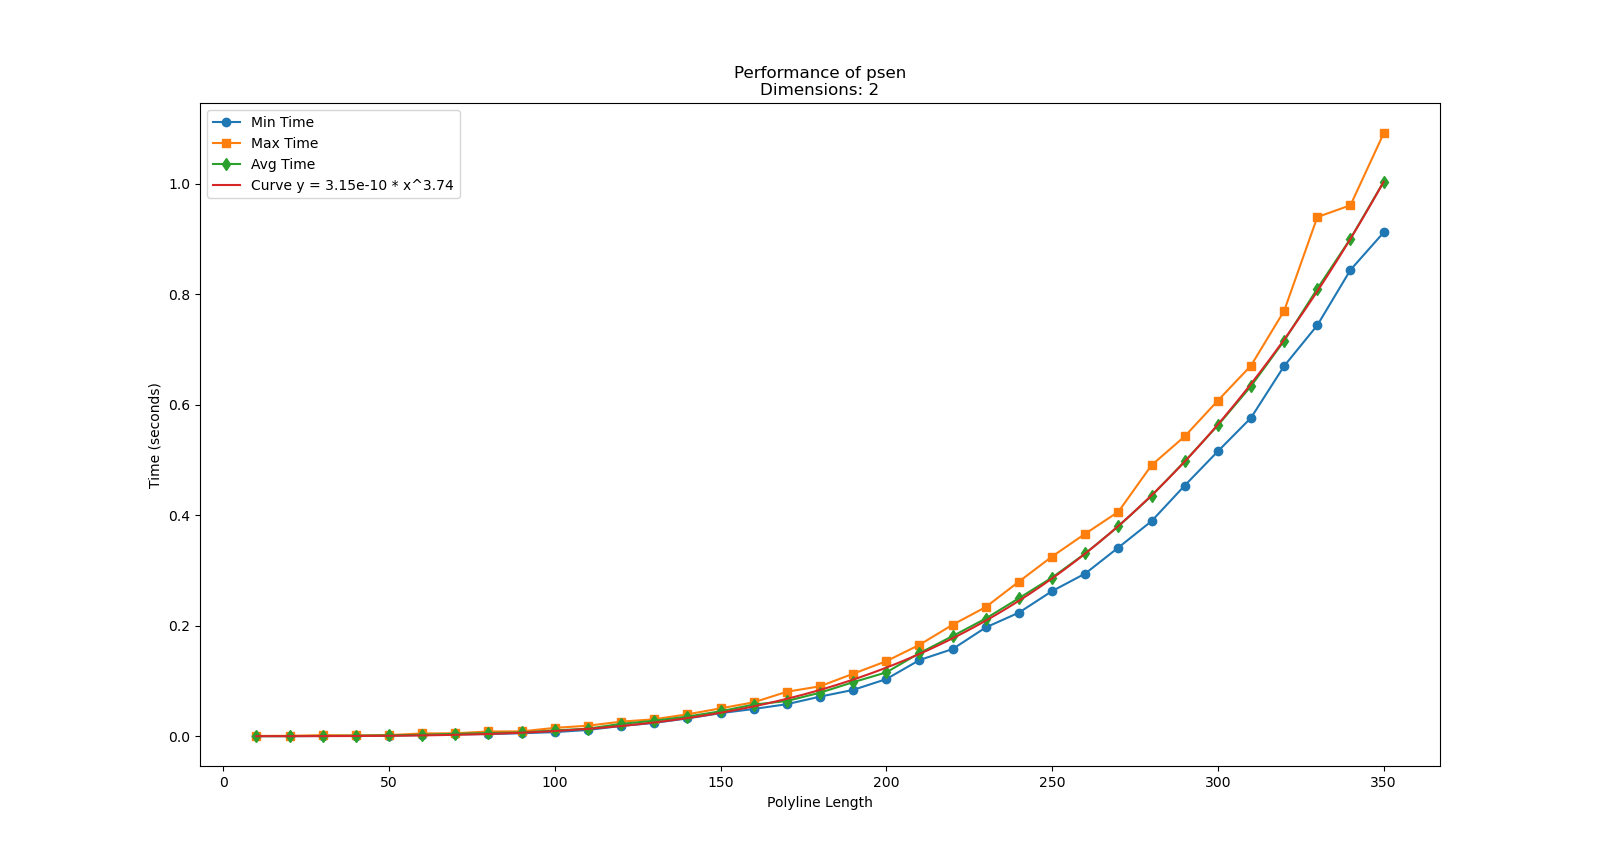
\includegraphics[scale=0.5, width=\linewidth]{figures/psen.png}
  \caption{Parallel, explicit for well-behaved polylines}
  \label{fig:psen}
\end{figure}

In \cref{fig:psen} we can already see the first surprising result that is is also confirmed by the other tests: Using the simple optimizations that we have outlined, the runtime is far better than the theoretical \(\O(n^6)\) for large simplifications to a sub-quartic, but super-cubic, runtime. We still want to mention that \(350\) is still a rather small size thus the runtime could grow worse than what these plots show. 

\begin{figure}[ht]
  \centering
  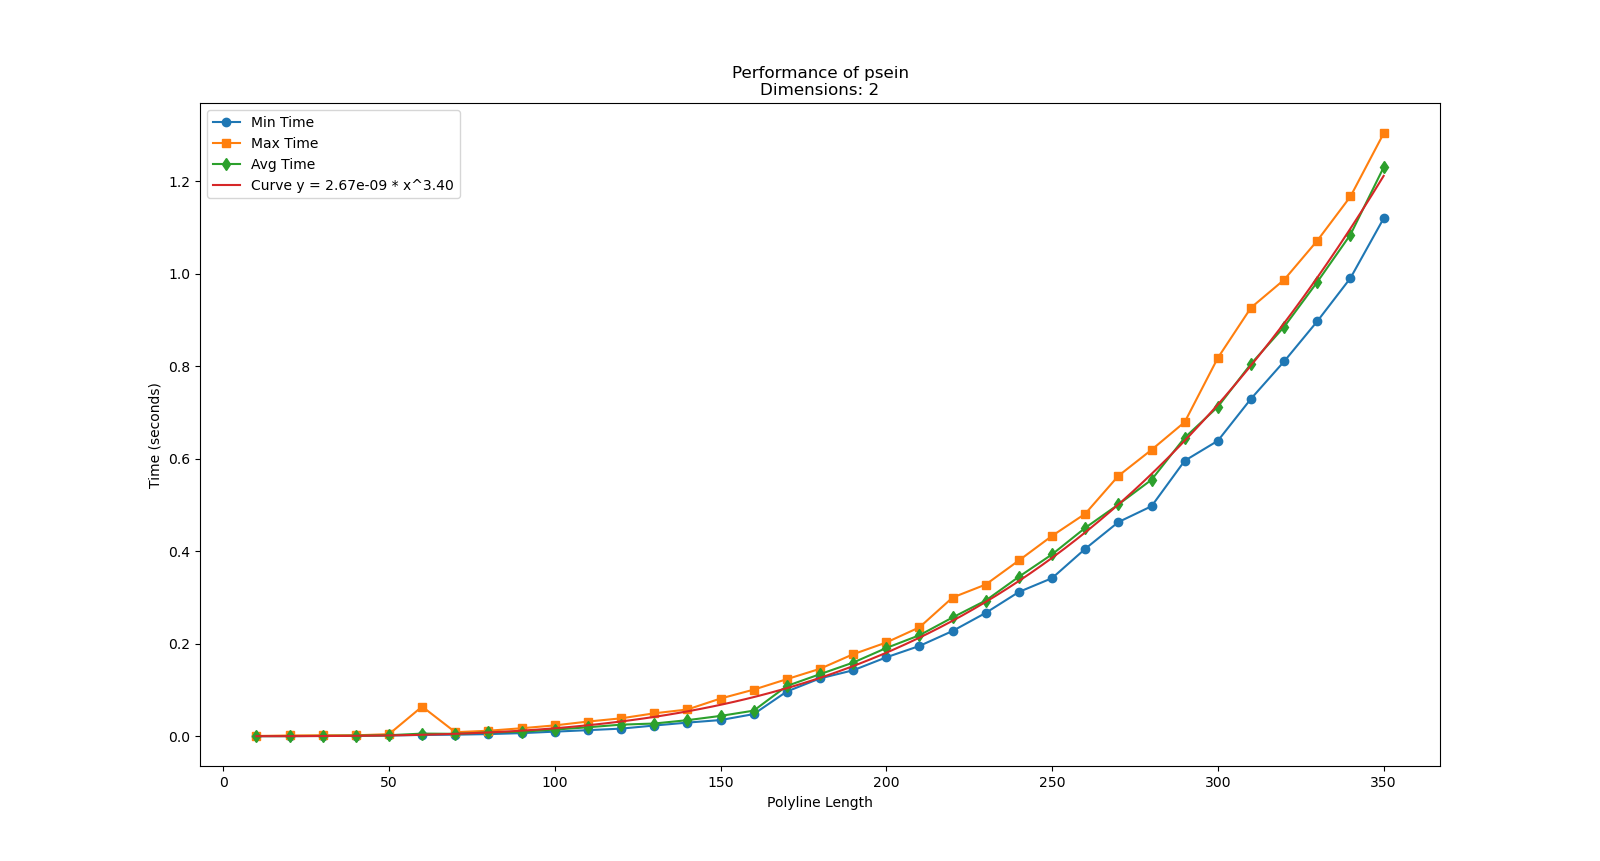
\includegraphics[scale=0.5, width=\linewidth]{figures/psein.png}
  \caption{Parallel, implicit for well-behaved polylines}
  \label{fig:psein}
\end{figure}

\begin{figure}[ht]
  \centering
  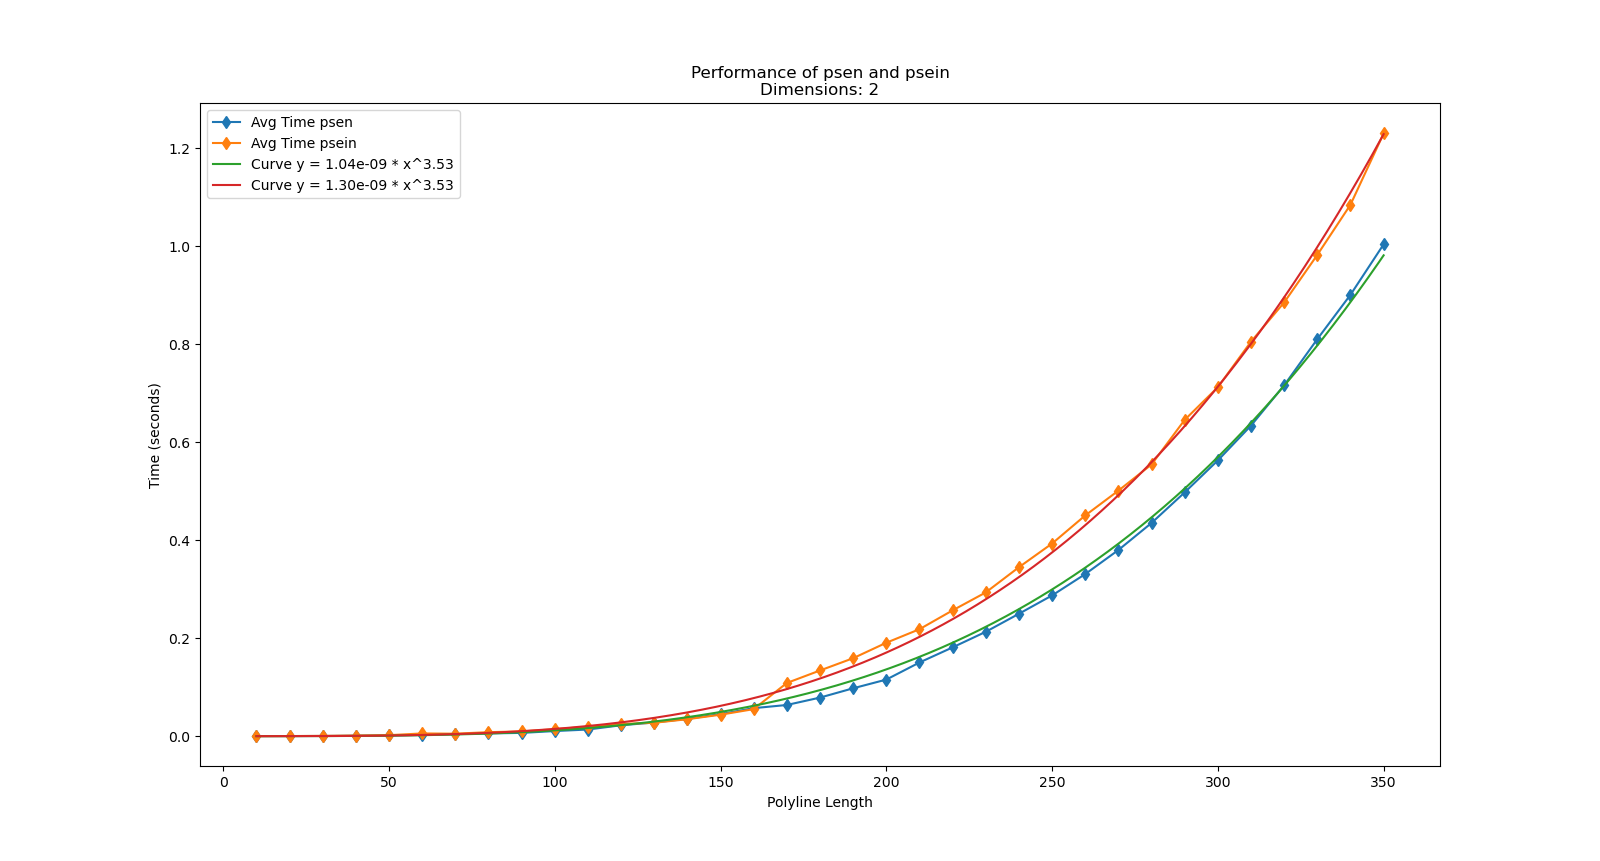
\includegraphics[scale=0.5, width=\linewidth]{figures/psen-psein.png}
  \caption{Parallel, both implicit and explicit for well-behaved polylines}
  \label{fig:psen-psein}
\end{figure}

The implicit approach, as can be seen in \cref{fig:psein} and in comparison with the explicit in \cref{fig:psen-psein} is about 20\% slower than the explicit algorithm. We suspect that is because of added complexity and checks in the implicit case which are harder to parallelize. Interestingly, there is a noticeable increase in the runtime from polyline of size \(160\) to \(170\). As the data points before form a rather smooth line as well as the ones after that point, it is unlikely that it is just an outlier. It could possibly be because of the chunksize for the parallelization or other intricacies of the parallelization that allow faster simplification for polylines of size smaller than \(170\).

\begin{figure}[ht]
  \centering
  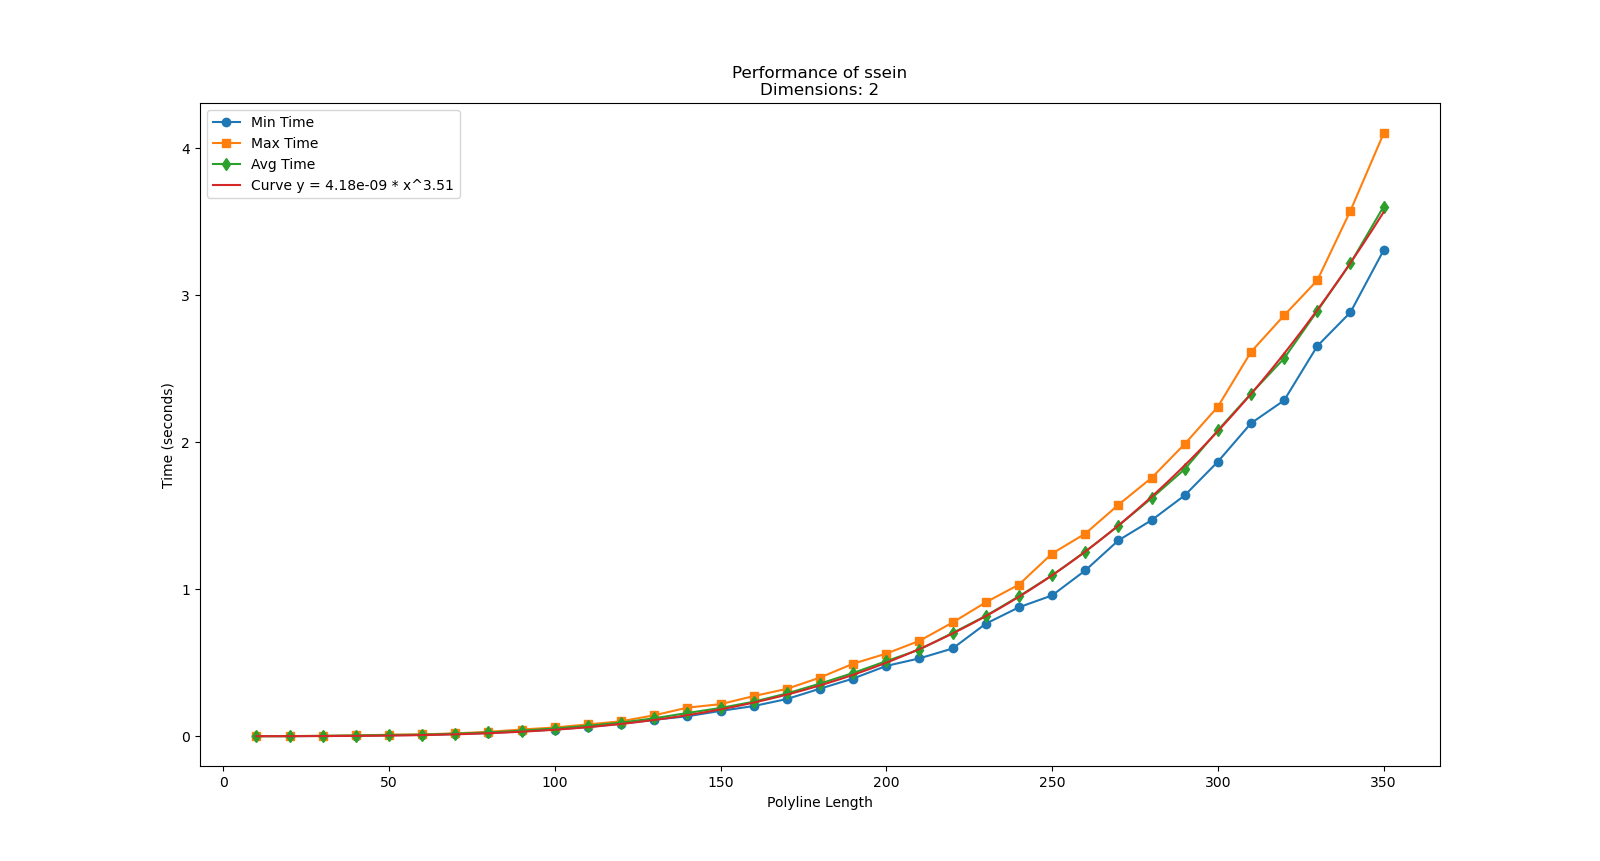
\includegraphics[scale=0.5, width=\linewidth]{figures/ssein.png}
  \caption{Sequential, explicit for well-behaved polylines}
  \label{fig:ssen}
\end{figure}

\begin{figure}[ht]
  \centering
  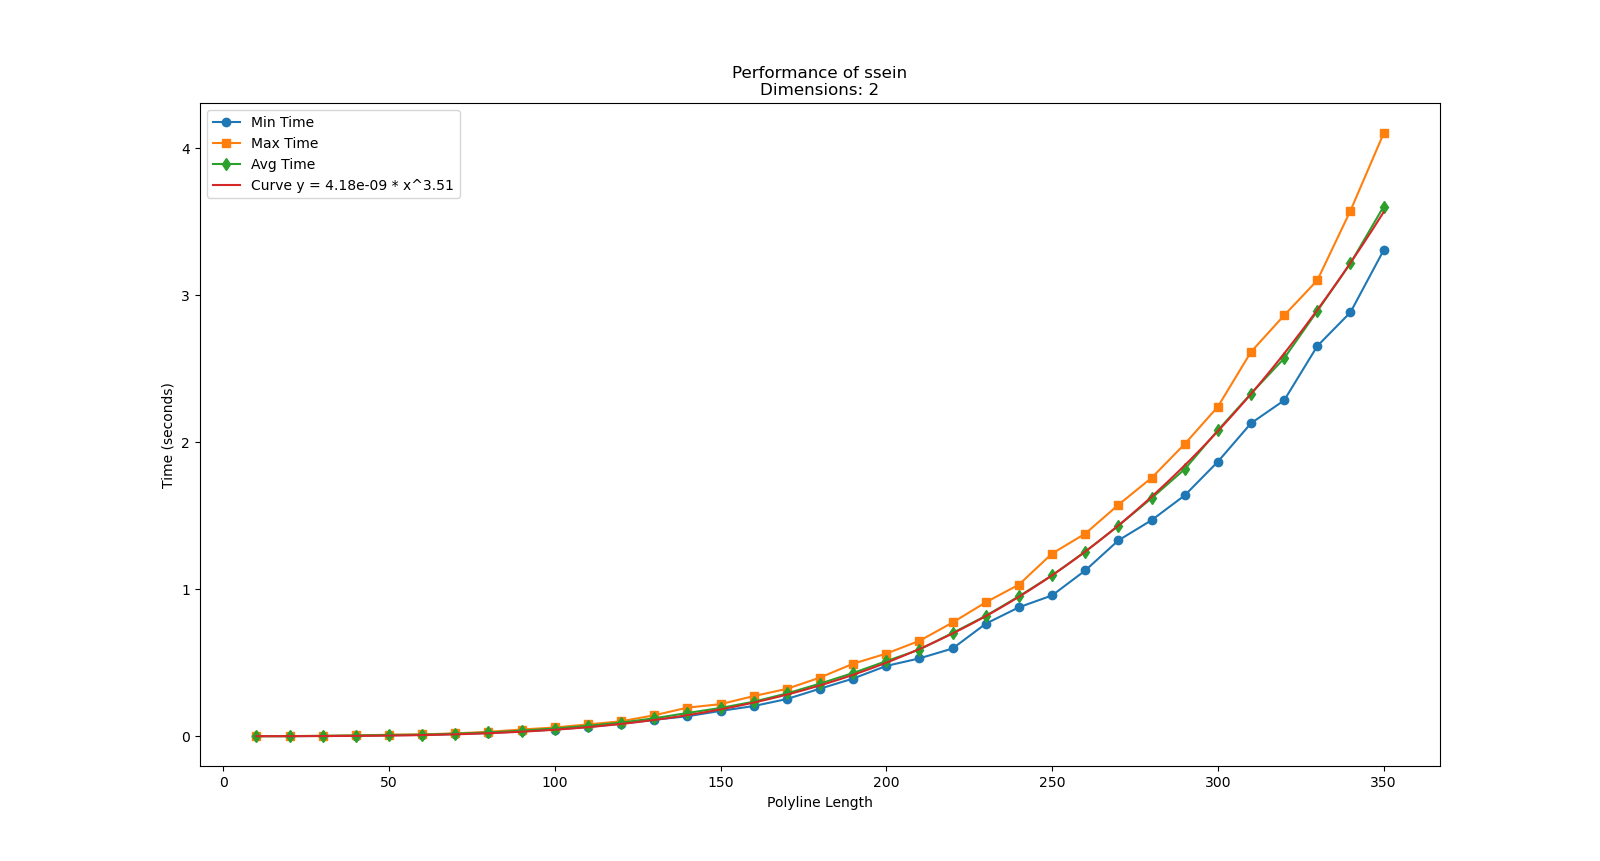
\includegraphics[scale=0.5, width=\linewidth]{figures/ssein.png}
  \caption{Sequential, implicit for well-behaved polylines}
  \label{fig:ssein}
\end{figure}

\begin{figure}[ht]
  \centering
  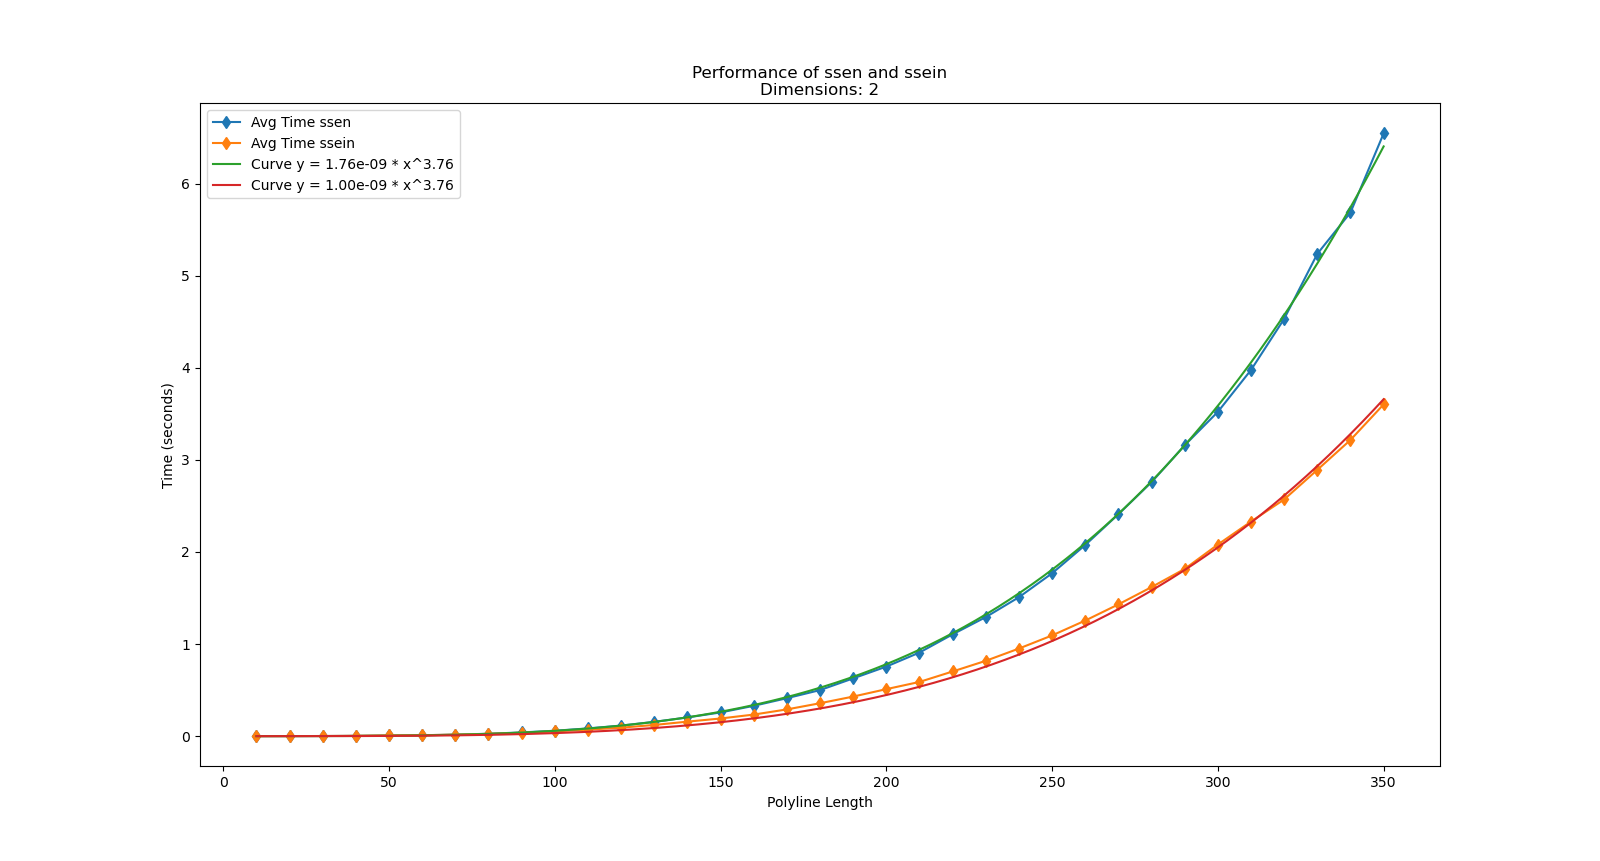
\includegraphics[scale=0.5, width=\linewidth]{figures/ssen-ssein.png}
  \caption{Sequential, both explicit and implicit for well-behaved polylines}
  \label{fig:ssen-ssein}
\end{figure}

The sequential algorithms in \cref{fig:ssen}, \cref{fig:ssein}, and \cref{fig:ssen-ssein}  do not feature such noticeable jumps providing evidence that they are caused by less optimal parallelization. Surprisingly, whereas the explicit implementation was clearly faster in the parallelized case, for the sequential implementation the implicit one prevails. The explicit implementation seems to be almost 80\% slower than the implicit one. This could be because of compiler optimizations as the implicit case subdivides the needed work into multiple steps that allow early returns and throughout the algorithm multiple values can be shared thus profitting from instruction scheduling. The explicit algorithm needs to compute the whole solution every time.

\begin{figure}[ht]
  \centering
  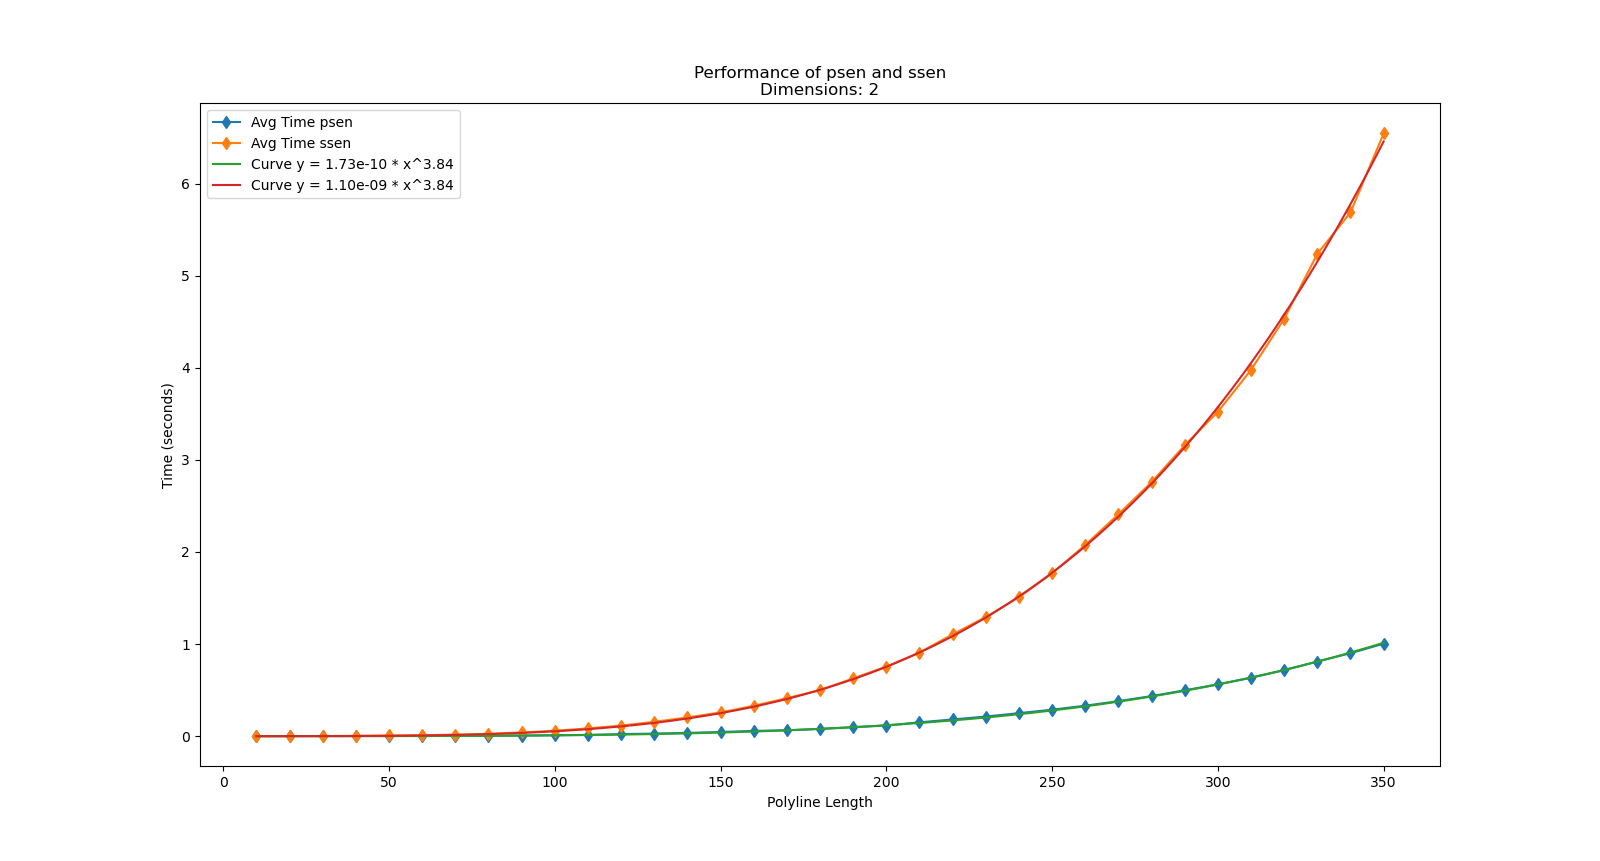
\includegraphics[scale=0.5, width=\linewidth]{figures/psen-ssen.png}
  \caption{Parallel and sequential, explicit for well-behaved polylines}
  \label{fig:psen-ssen}
\end{figure}

\begin{figure}[ht]
  \centering
  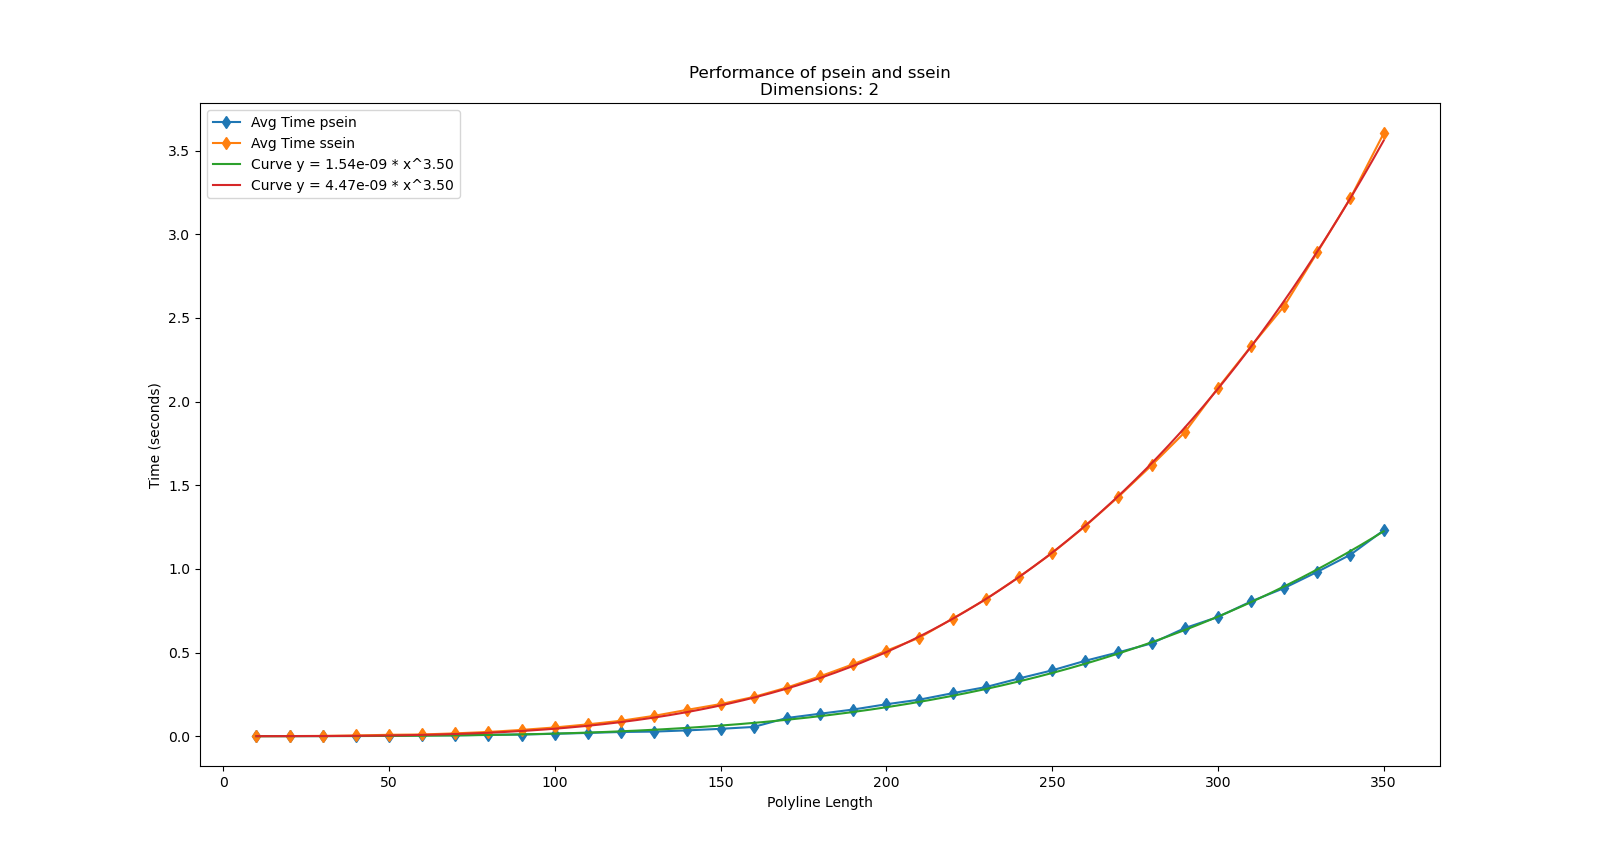
\includegraphics[scale=0.5, width=\linewidth]{figures/psein-ssein.png}
  \caption{Parallel and sequential, implicit for well-behaved polylines}
  \label{fig:psein-ssein}
\end{figure}

Comparing the sequential and parallel algorithm, in \cref{fig:psen-ssen} we notice that the explicit algorithm is about \(6.5\) times faster parallelized, the implicit algorithm in \cref{fig:psein-ssein} only gains a sppedup of a factor of \(3\). 

Having seen the different implementations of the algorithm, we now investigate the effect of the data.

\begin{figure}[ht]
  \centering
  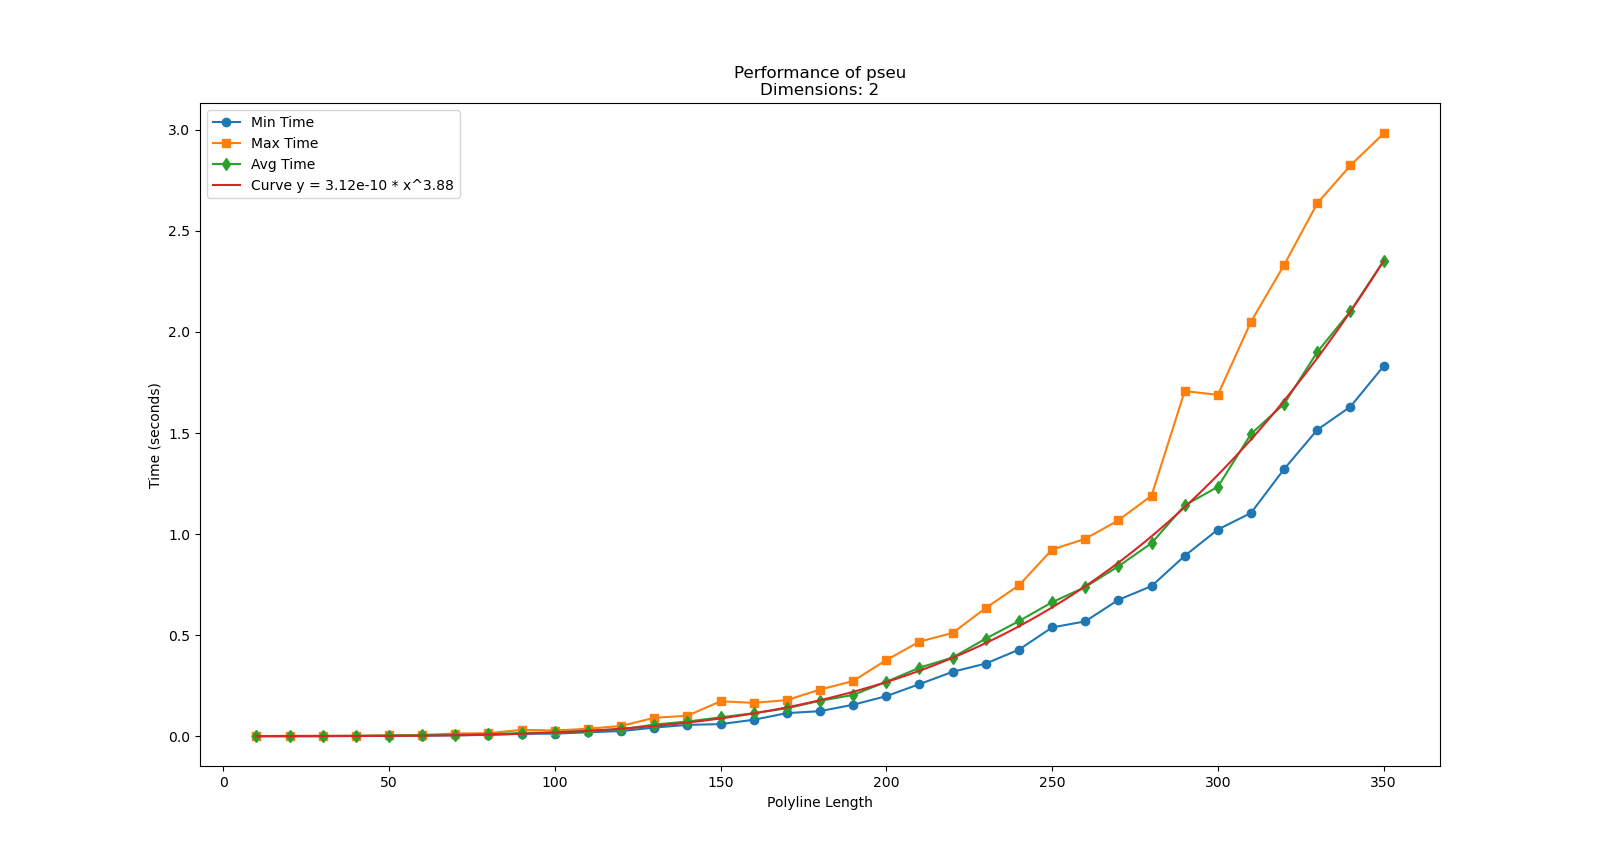
\includegraphics[scale=0.5, width=\linewidth]{figures/pseu.png}
  \caption{Parallel, explicit for non-well-behaved polylines}
  \label{fig:pseu}
\end{figure}

\begin{figure}[ht]
  \centering
  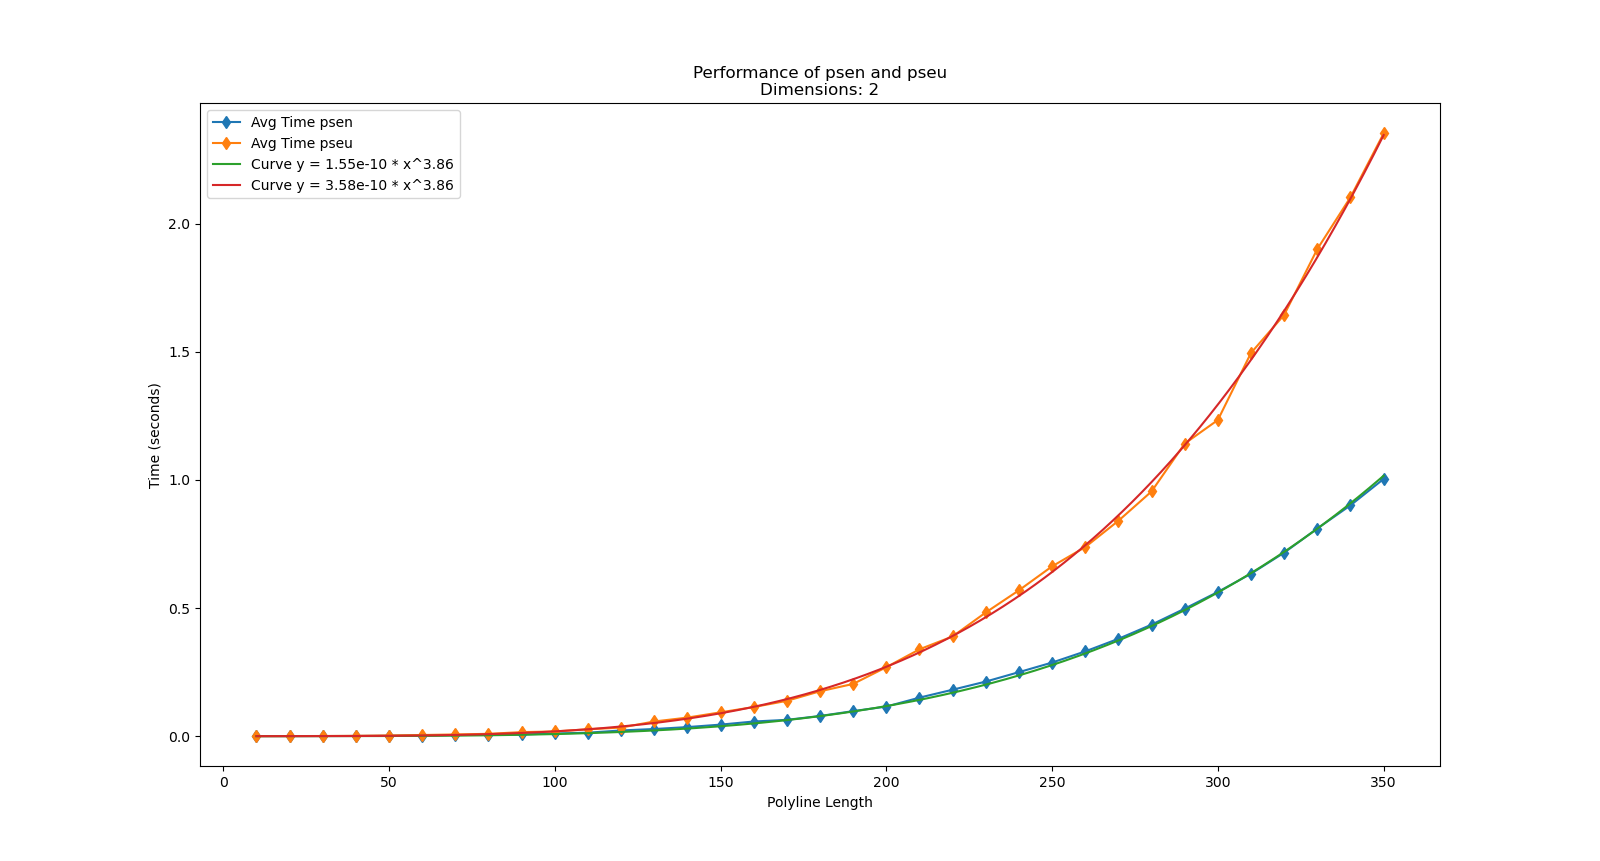
\includegraphics[scale=0.5, width=\linewidth]{figures/psen-pseu.png}
  \caption{Parallel, explicit for well-behaved and non-well-behaved polylines}
  \label{fig:psen-pseu}
\end{figure}

Looking at the maximum and minimum time in \cref{fig:pseu} and especially \cref{fig:pseiu} we can see that there is more variance than in the well-behaved polylines showing that non-well-behaved can take longer than well-behaved ones even if they are smaller. \cref{fig:psen-pseu} and \cref{fig:psein-pseiu} compares the non-well-behaved and the well-behaved ones directly showing that they take more than twice as long to process.

\begin{figure}[ht]
  \centering
  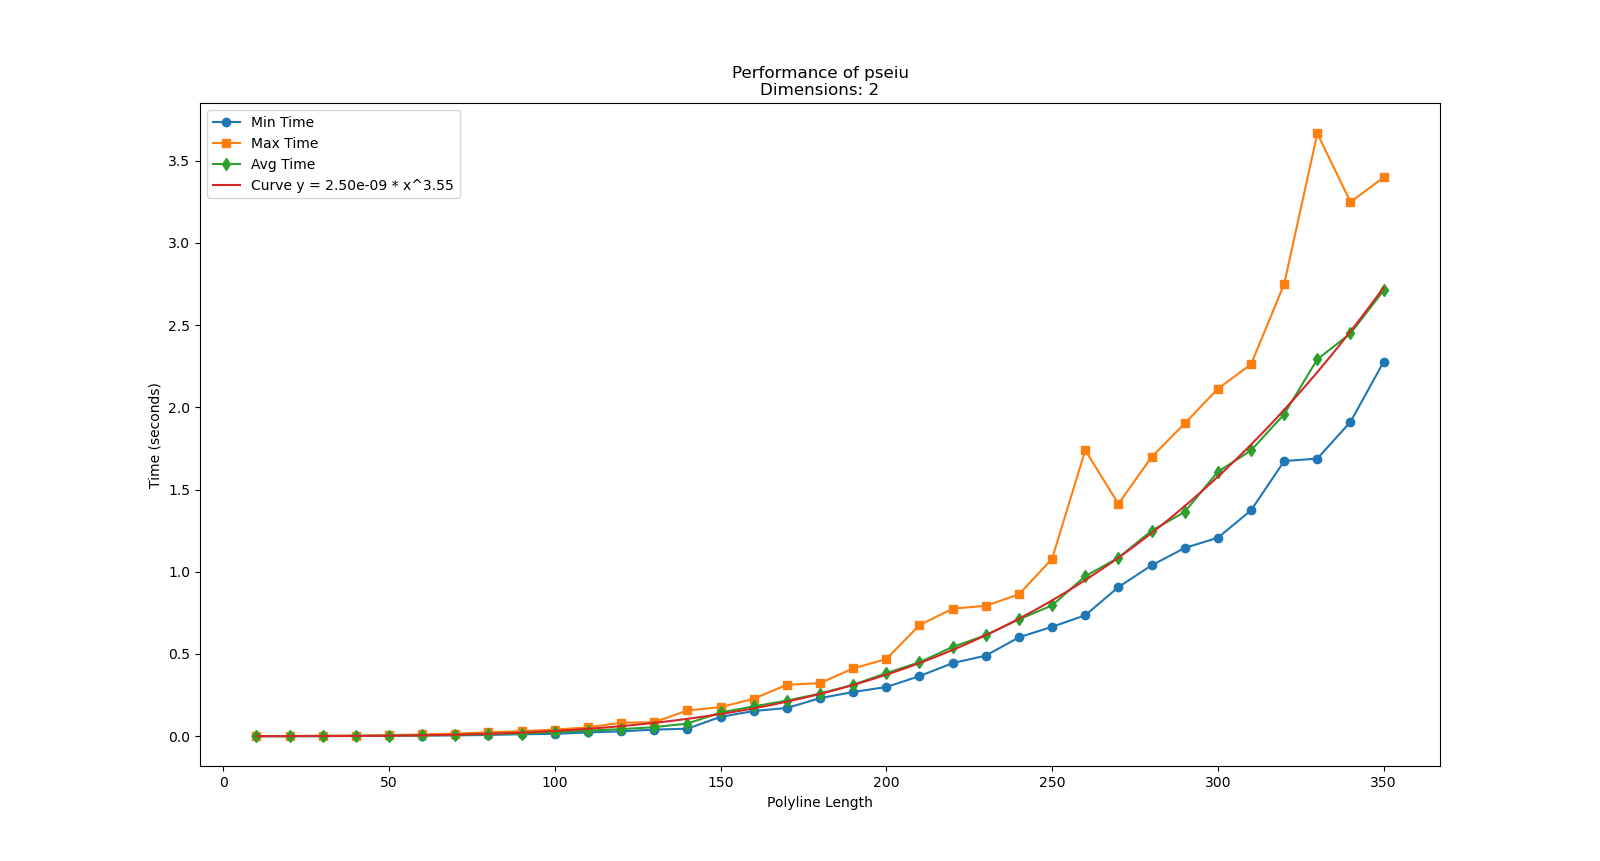
\includegraphics[scale=0.5, width=\linewidth]{figures/pseiu.png}
  \caption{Parallel, implicit for non-well-behaved polylines}
  \label{fig:pseiu}
\end{figure}

\begin{figure}[ht]
  \centering
  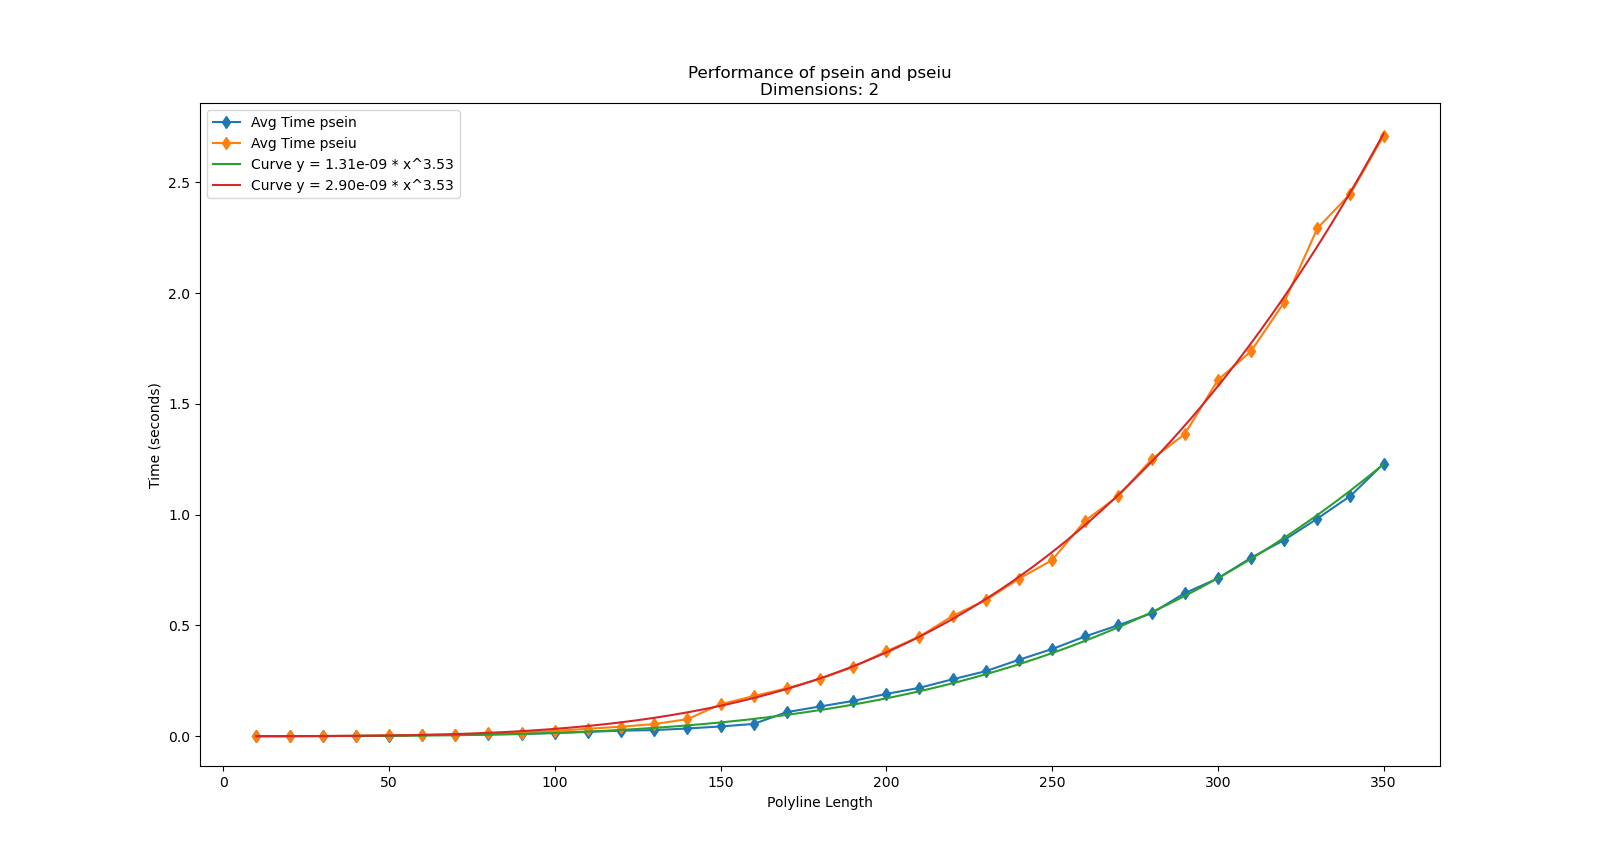
\includegraphics[scale=0.5, width=\linewidth]{figures/psein-pseiu.png}
  \caption{Parallel, implicit for well-behaved and non-well-behaved polylines}
  \label{fig:psein-pseiu}
\end{figure}

Finally, we cover the effect of our optimizations. We test all of them on well-behaved polylines with parallelization for polylines of length upto \(150\).
\cref{fig:psenn} and \cref{fig:pseinn} are exhibit very smooth behaviour with little variation as is expected because they perform all computations for all polylines with the only difference being the size of the simplification. We again remind that the regression lines do not capture the full behaviour of the algorithms because of the few data samples. The runtime for the unoptimized version \emph{cannot} be faster than \(O(n^5)\) and as we always used a rather small \(\varepsilon\) resulting in large simplifications, the actual runtime is of the order \(\O(n^6)\).
Without the reachability optimization, the runtimes also look rather smooth, especially for the implicit algorithm in \cref{fig:pseinr} while the explicit version in \cref{fig:psenr} has more variance.  
The minimality optimizations, on the other hand, exhibit rather wild behavior with very noticeable outliers for both. We are unsure whether that is caused by some implementation bug, external circumstances, or an inherent property of the polyline. Note that the outliers are different for the explicit and implicit case as the data is generated for each separately. 

The outliers may be more highlighted because of less data and only testing for smaller test cases so it can be questioned how representative they are. 

Lastly comparing the optimizations against each other we can see that in the explicit case, any of the three optimization suffices to get the speedup, while the implicit case requires the reachability optimization however we are unsure how it is possible that the case with no optimizations at all is faster than the one that only omits the reachability optimization. It may be that the needed comparisons for the other optimizations take more time than they save but why there is such an extreme difference between the explicit and implicit case in this regards is unclear. 

It can be easily seen that the optimizations are necessary for reasonable runtimes, however which ones to use is unclear. Theoretically, the local minimality optimization is unnecessary when using the global one as the local version can only ever occur once per \((i, j)\) pair. This is because it finds the minimum which causes the global optimization to skipp all further iterations over the same pair meaning the local optimization can never occur again for the same \(i, j\). This could explain why omitting the local optimization seems to be faster than having it while omitting only the global one is slower. The reason that omitting the global minimality optimzation is not that much slower than having it could be because we only tested well-behaved polylines which may allow finding the minimum value more easily and thus allowing the local optimization to act as the global one. 

It is surprising that even without optimizations we can perform the algorithm somewhat comfortably on polylines of size \(150\) as \(150^5 \approx 7.5 \cdot 10^{10}\) which is the amount of steps the runtime suggests. We suspect that it still runs rather good is because the individual computations are fast arithmetical ones and the algorithm itself is structurally rather simple with little overhead. On our hardware we have a clock speed of about \(4.38 \cdot 10^9\) cycles per second. Accounting for parallelization as well as low constants factors that we would expect for the algorithm, this matches the observed execution time.

\begin{figure}[ht]
  \centering
  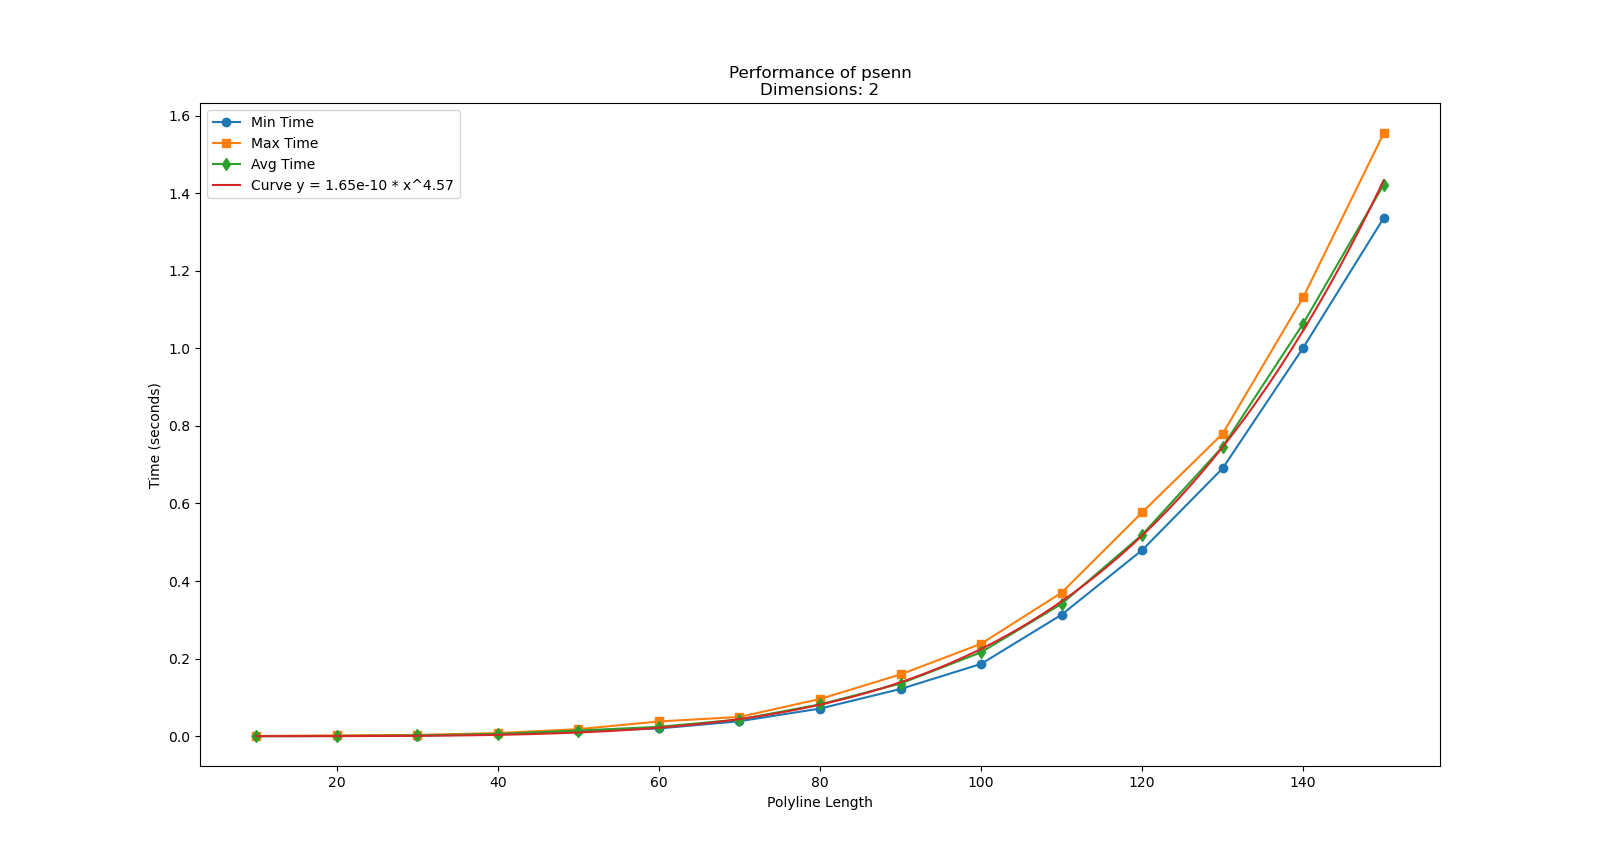
\includegraphics[scale=0.5, width=\linewidth]{figures/psenn.png}
  \caption{Parallel, explicit for well-behaved with no optimizations}
  \label{fig:psenn}
\end{figure}

\begin{figure}[ht]
  \centering
  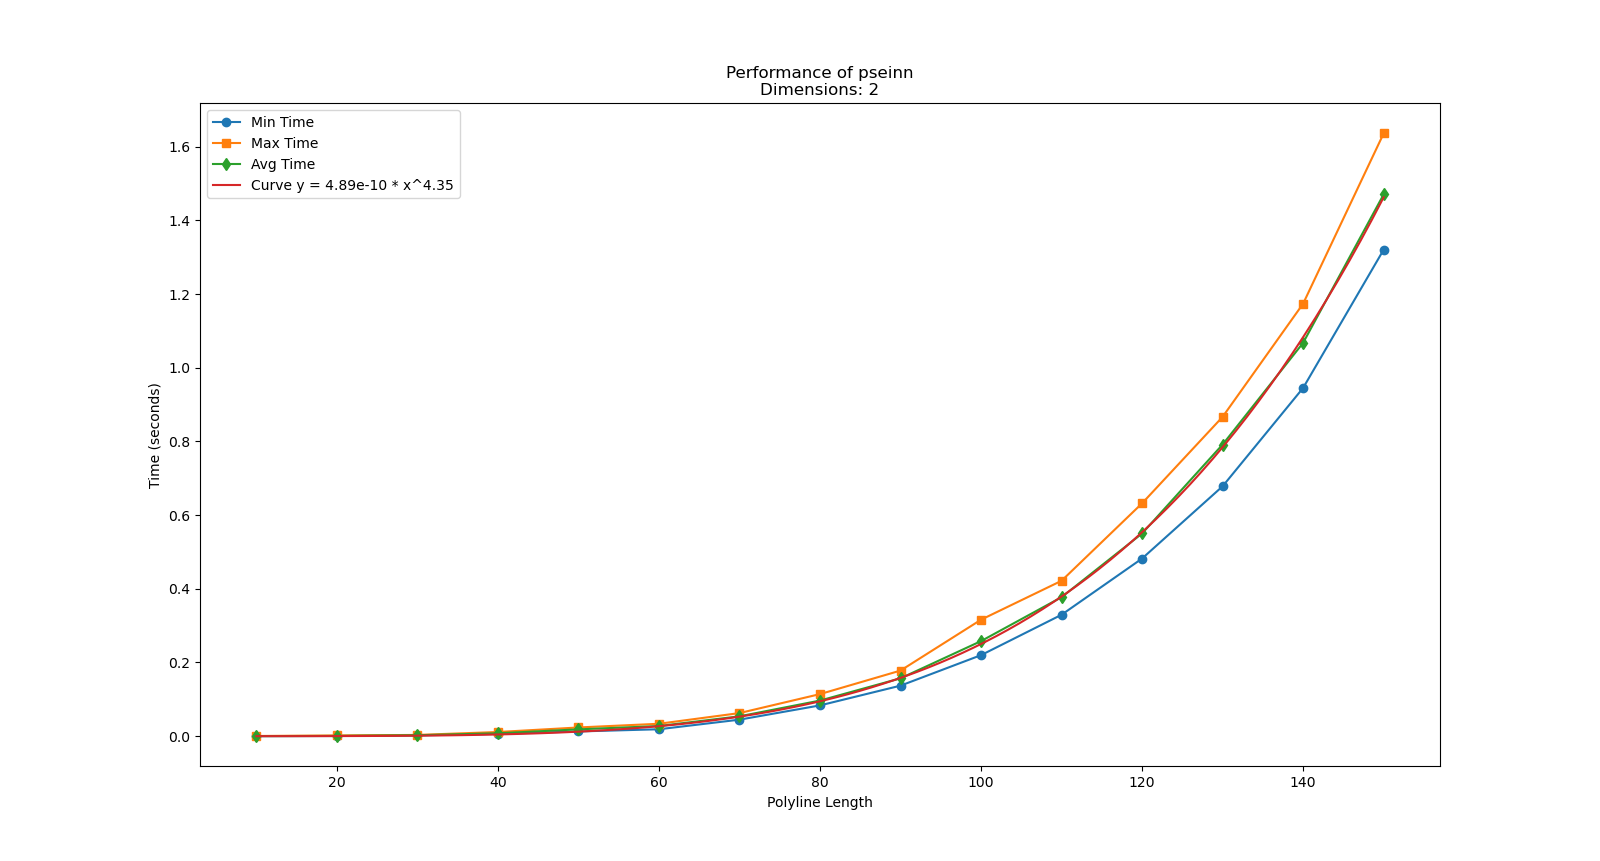
\includegraphics[scale=0.5, width=\linewidth]{figures/pseinn.png}
  \caption{Parallel, implicit for well-behaved with no optimizations}
  \label{fig:pseinn}
\end{figure}

\begin{figure}[ht]
  \centering
  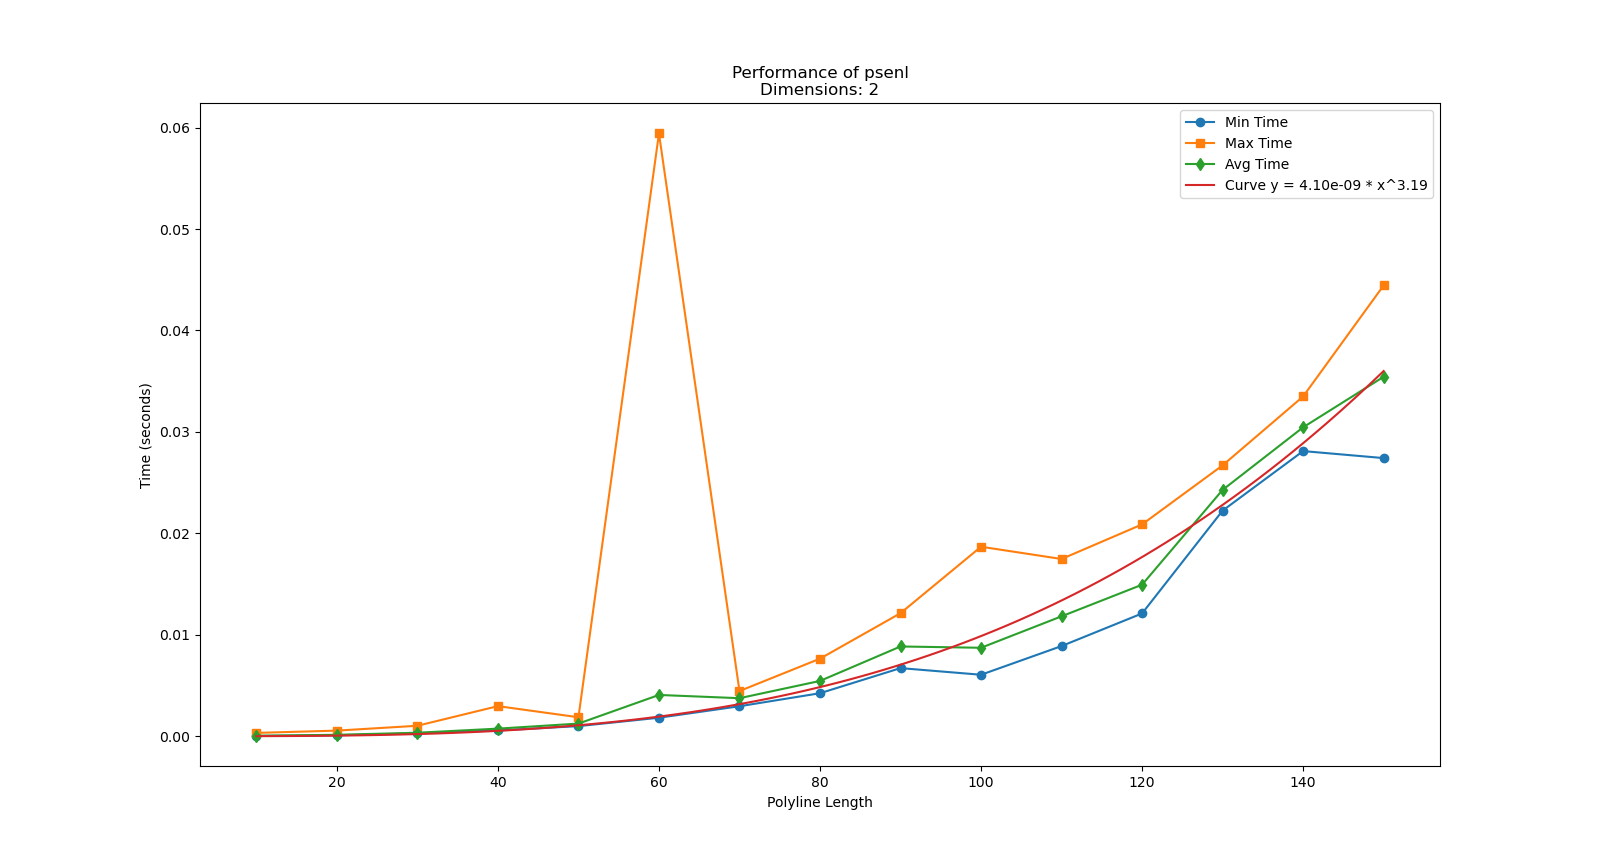
\includegraphics[scale=0.5, width=\linewidth]{figures/psenl.png}
  \caption{Parallel, explicit for well-behaved without local minimality optimization}
  \label{fig:psenl}
\end{figure}

\begin{figure}[ht]
  \centering
  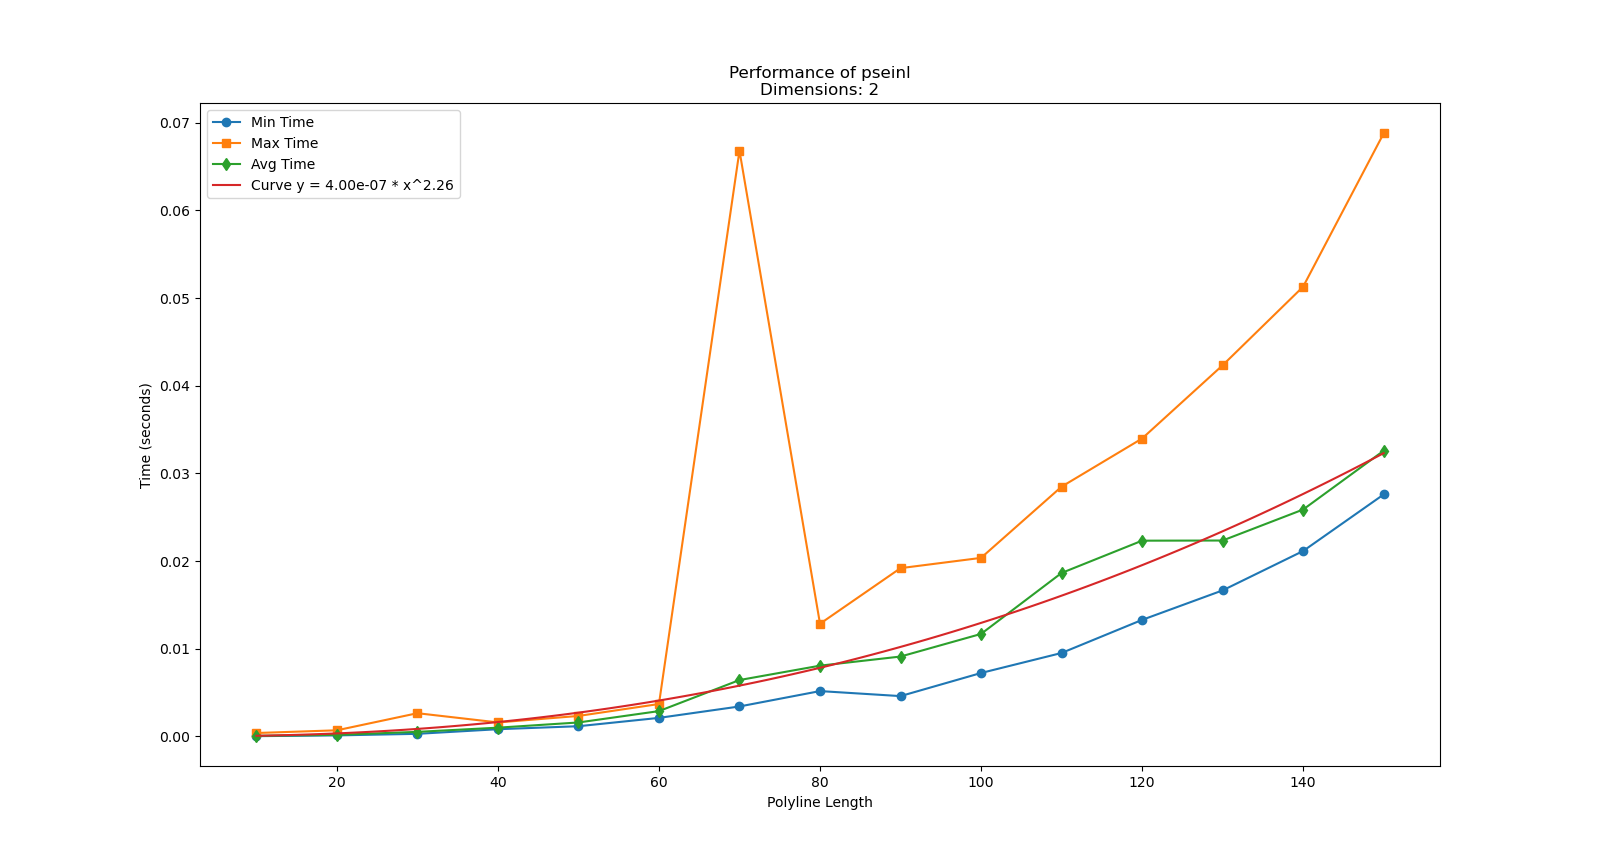
\includegraphics[scale=0.5, width=\linewidth]{figures/pseinl.png}
  \caption{Parallel, implicit for well-behaved without local minimality optimization}
  \label{fig:pseinl}
\end{figure}

\begin{figure}[ht]
  \centering
  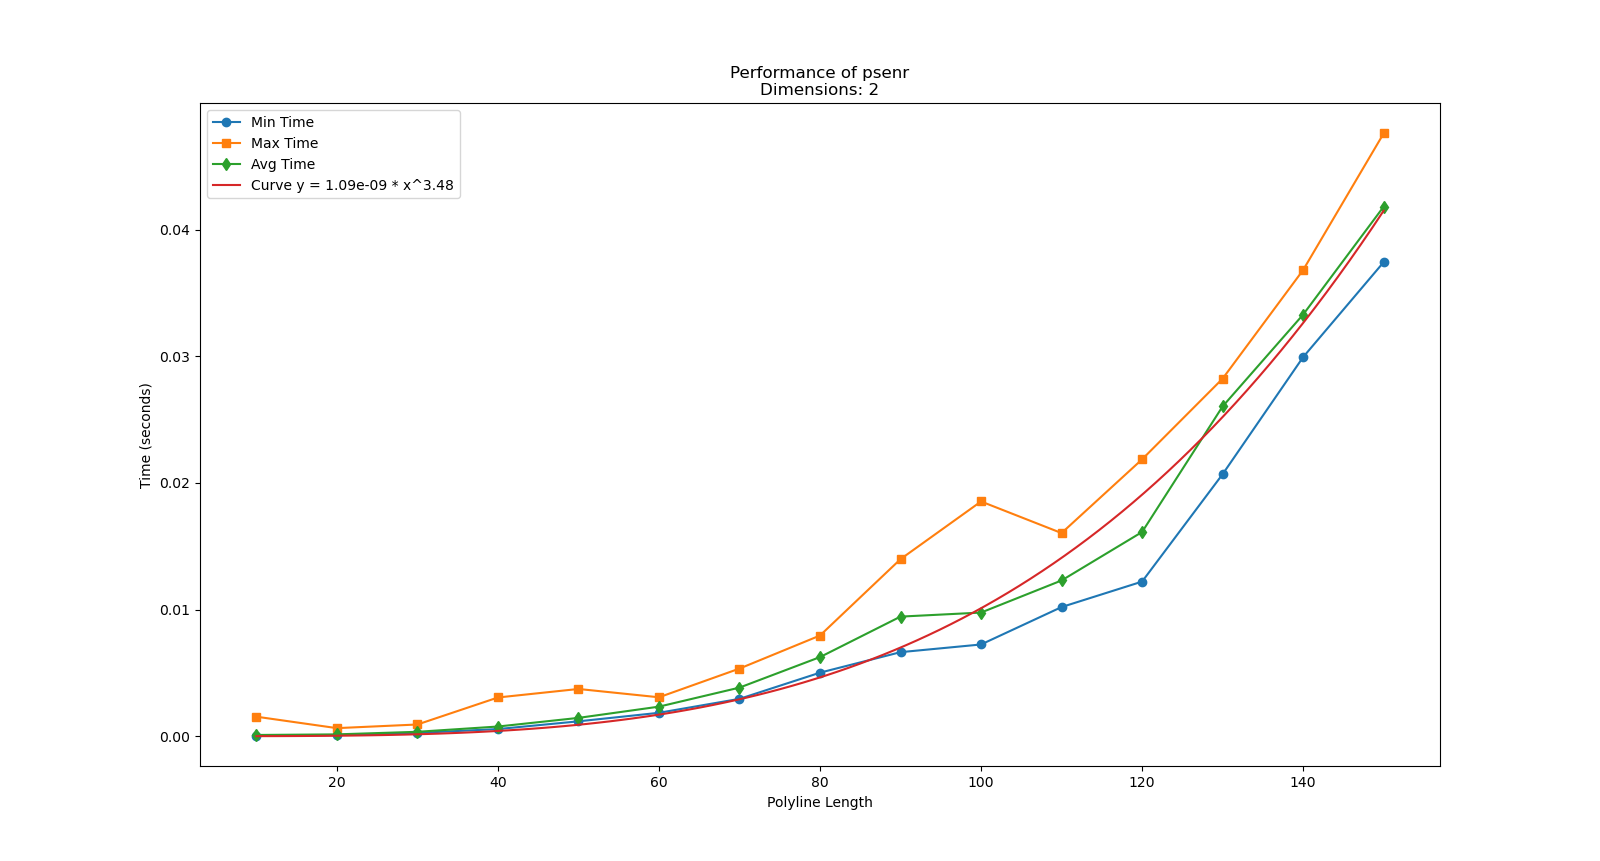
\includegraphics[scale=0.5, width=\linewidth]{figures/psenr.png}
  \caption{Parallel, explicit for well-behaved without reachability optimization}
  \label{fig:psenr}
\end{figure}

\begin{figure}[ht]
  \centering
  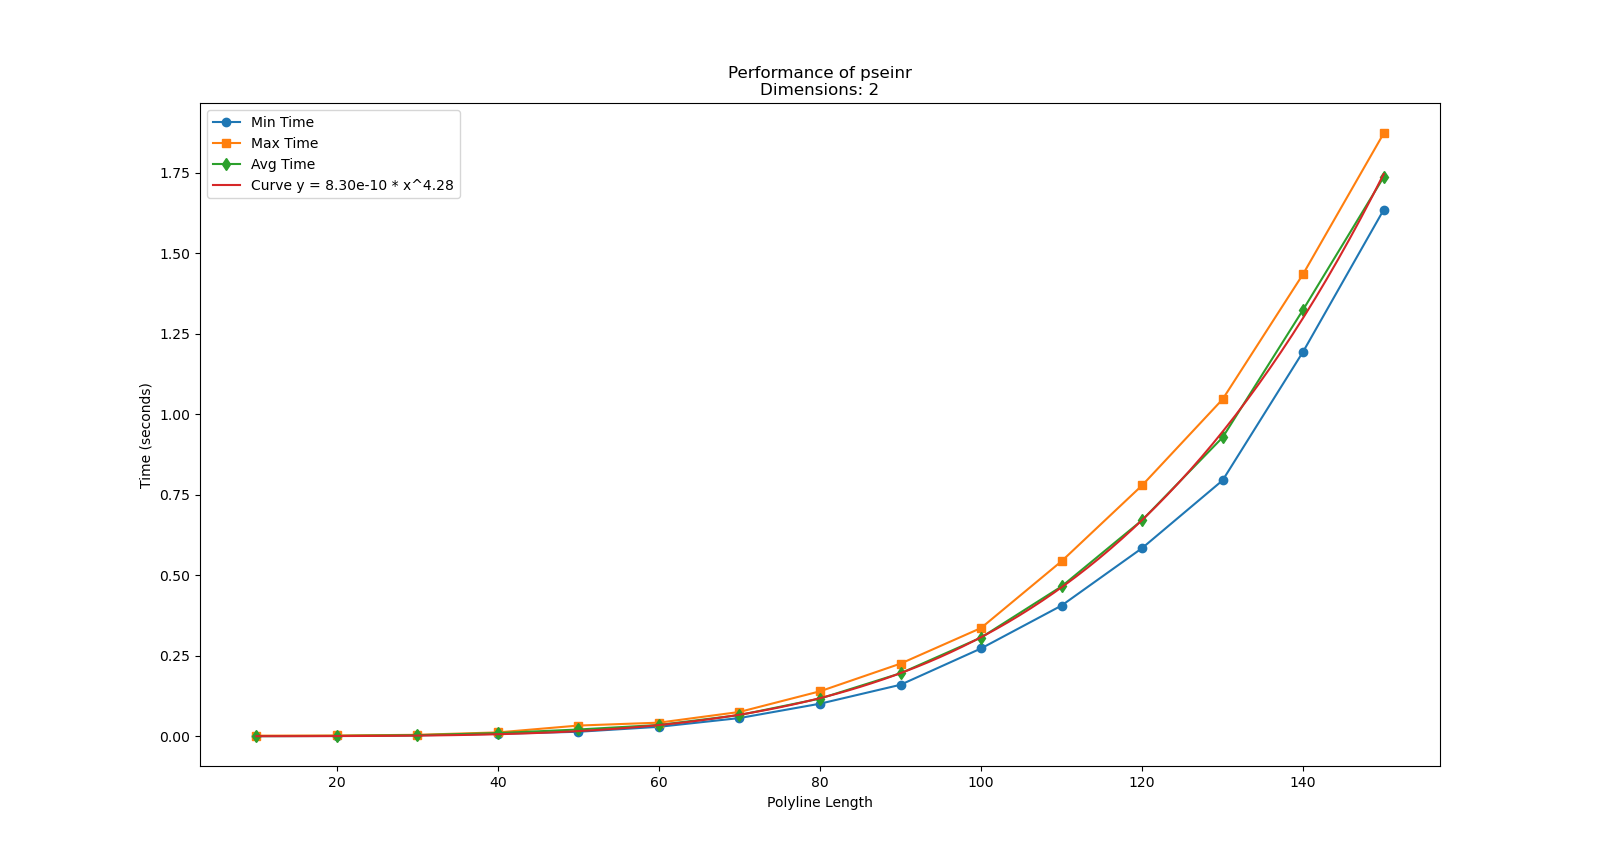
\includegraphics[scale=0.5, width=\linewidth]{figures/pseinr.png}
  \caption{Parallel, implicit for well-behaved without reachability optimization}
  \label{fig:pseinr}
\end{figure}

\begin{figure}[ht]
  \centering
  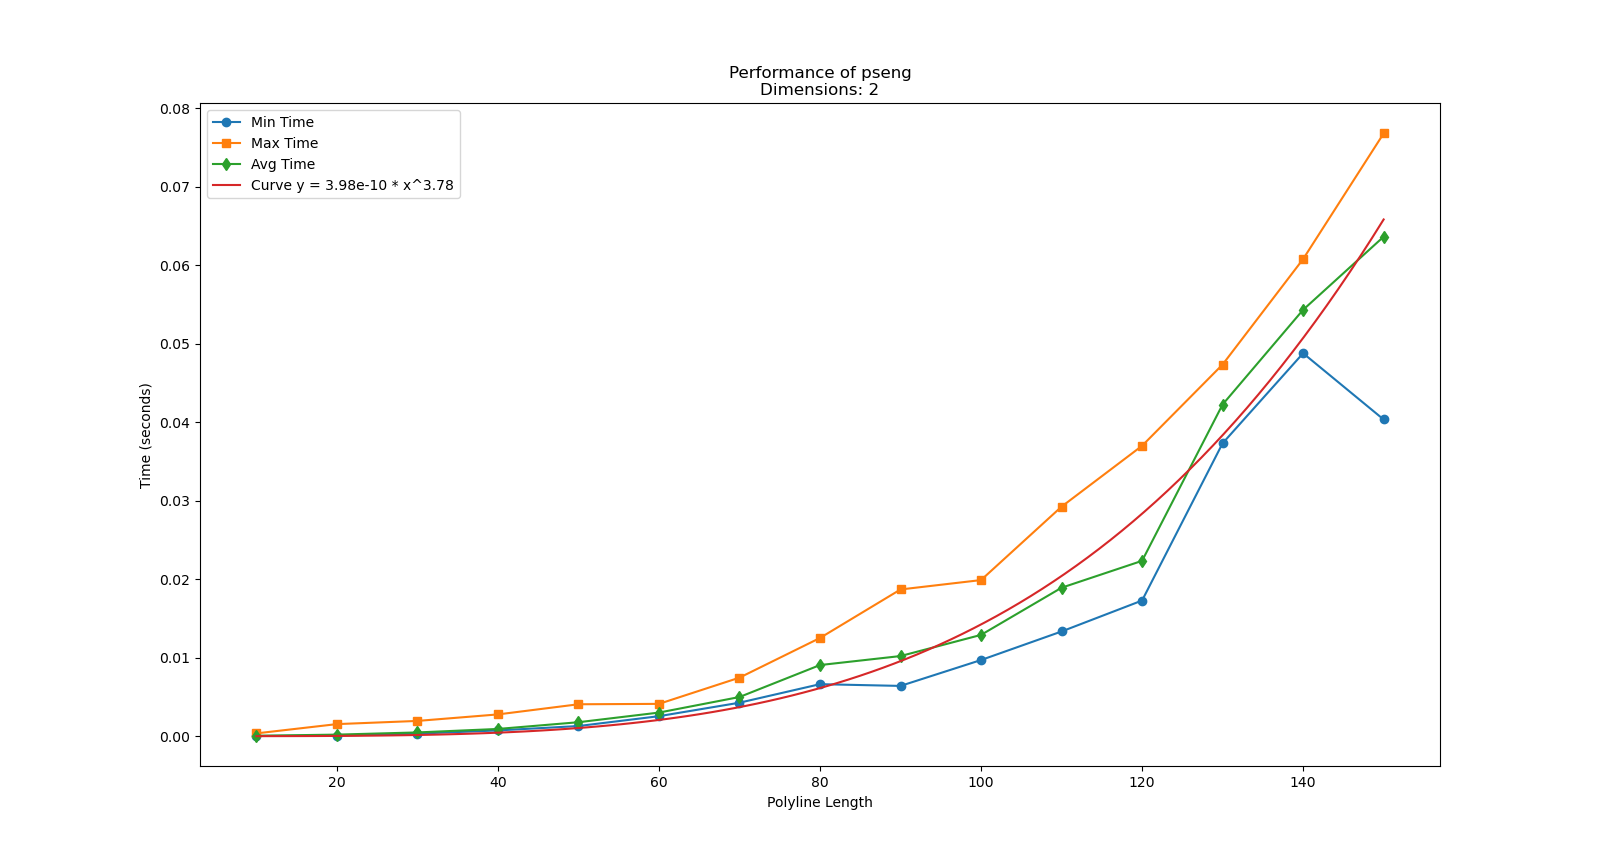
\includegraphics[scale=0.5, width=\linewidth]{figures/pseng.png}
  \caption{Parallel, explicit for well-behaved without global minimality optimization}
  \label{fig:pseng}
\end{figure}

\begin{figure}[ht]
  \centering
  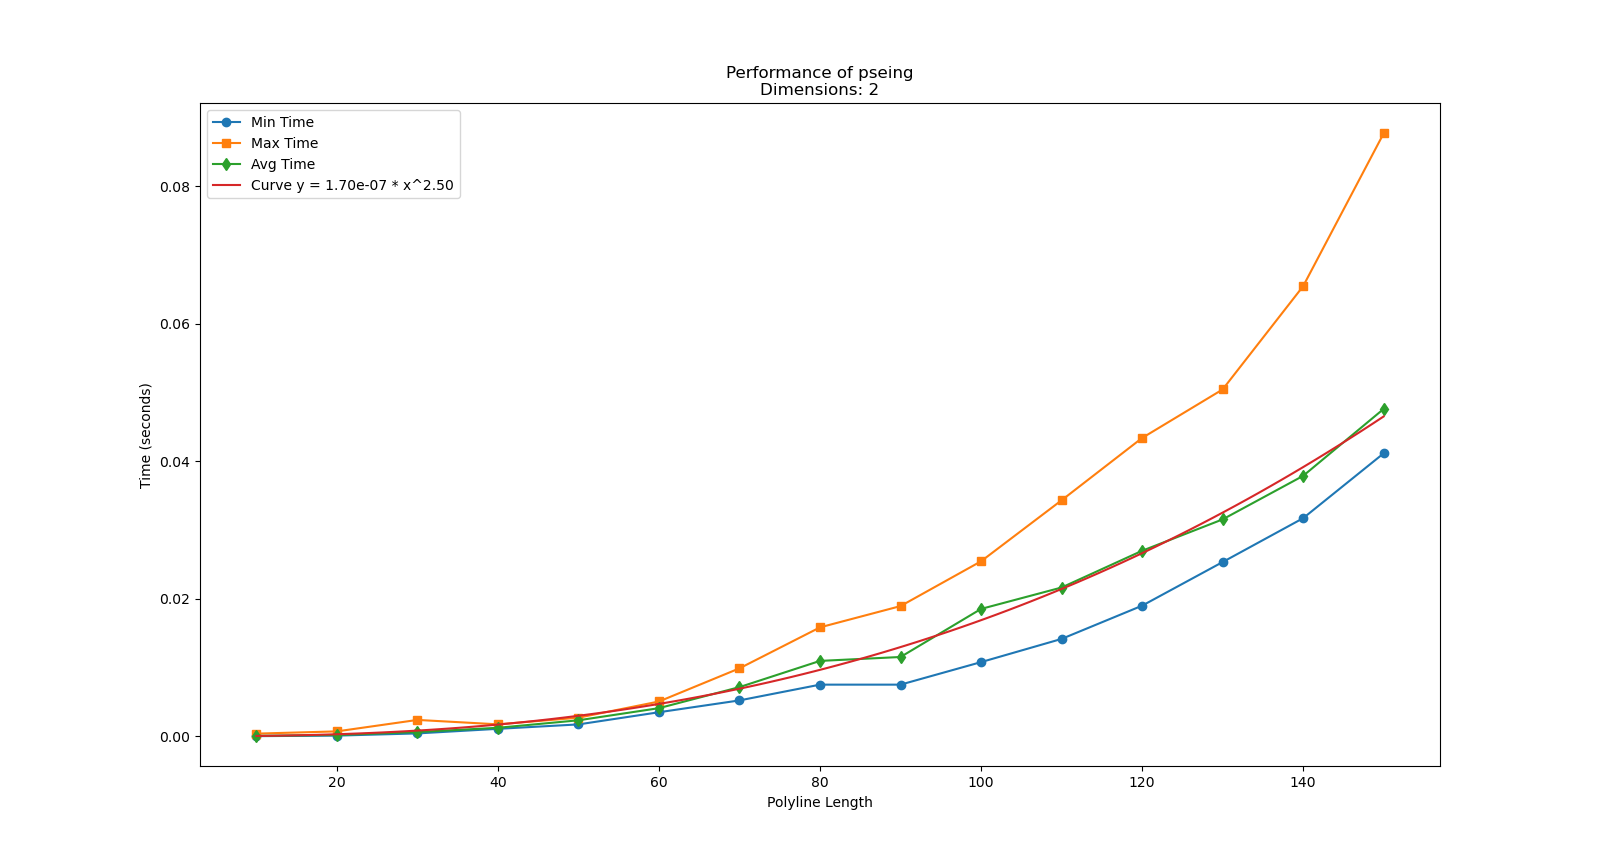
\includegraphics[scale=0.5, width=\linewidth]{figures/pseing.png}
  \caption{Parallel, implicit for well-behaved without global minimality optimization}
  \label{fig:pseing}
\end{figure}

\begin{figure}[ht]
  \centering
  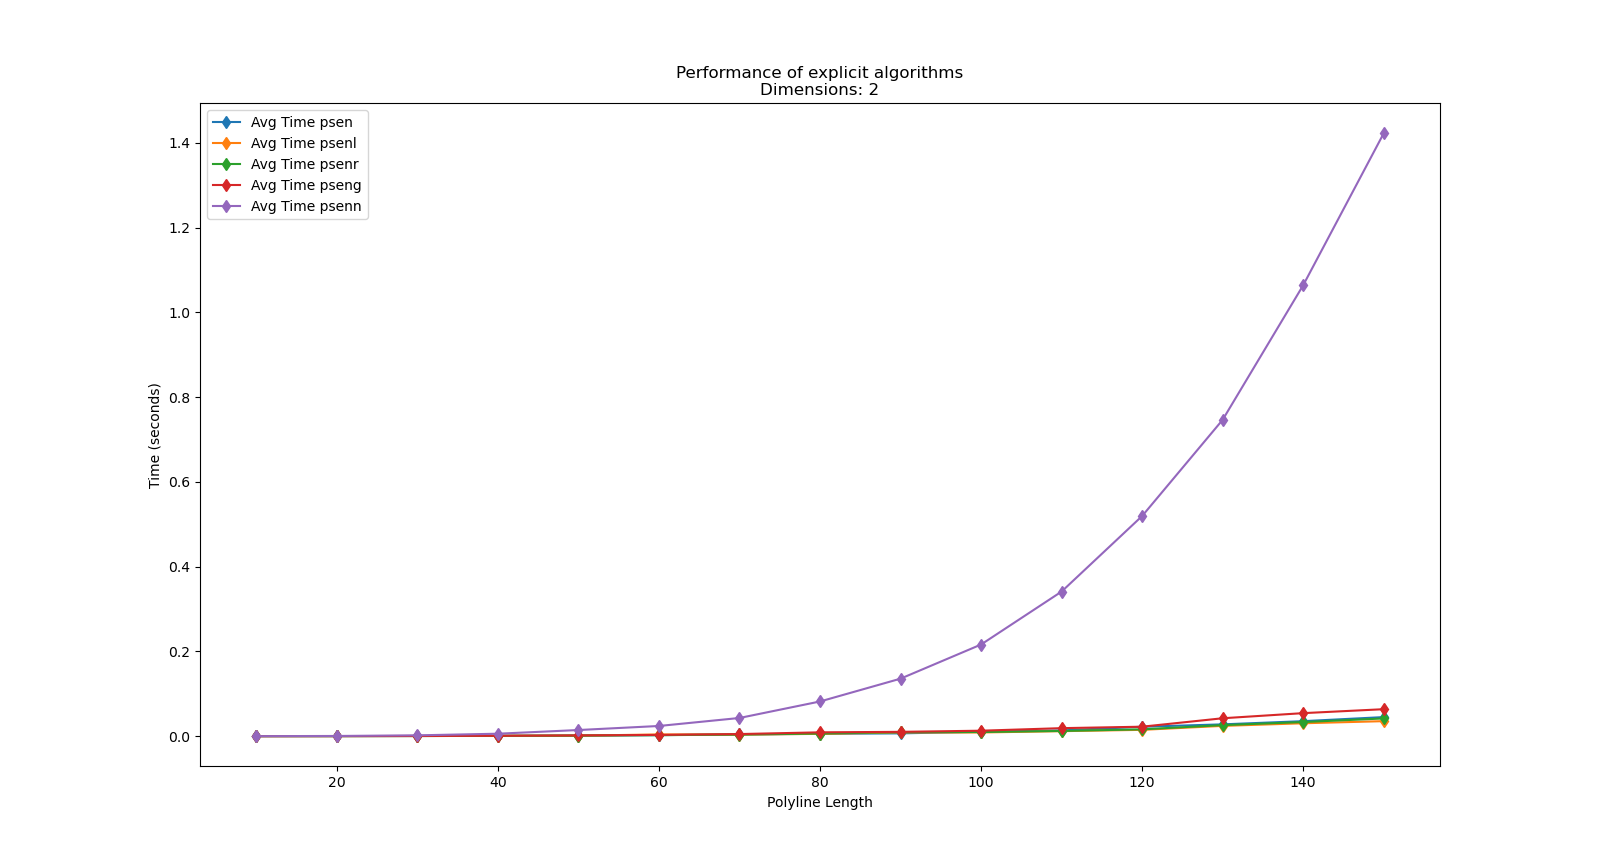
\includegraphics[scale=0.5, width=\linewidth]{figures/psen-opt1.png}
  \caption{Parallel, explicit for well-behaved polylines, comparison of optimizations}
  \label{fig:psen-opt1}
\end{figure}

\begin{figure}[ht]
  \centering
  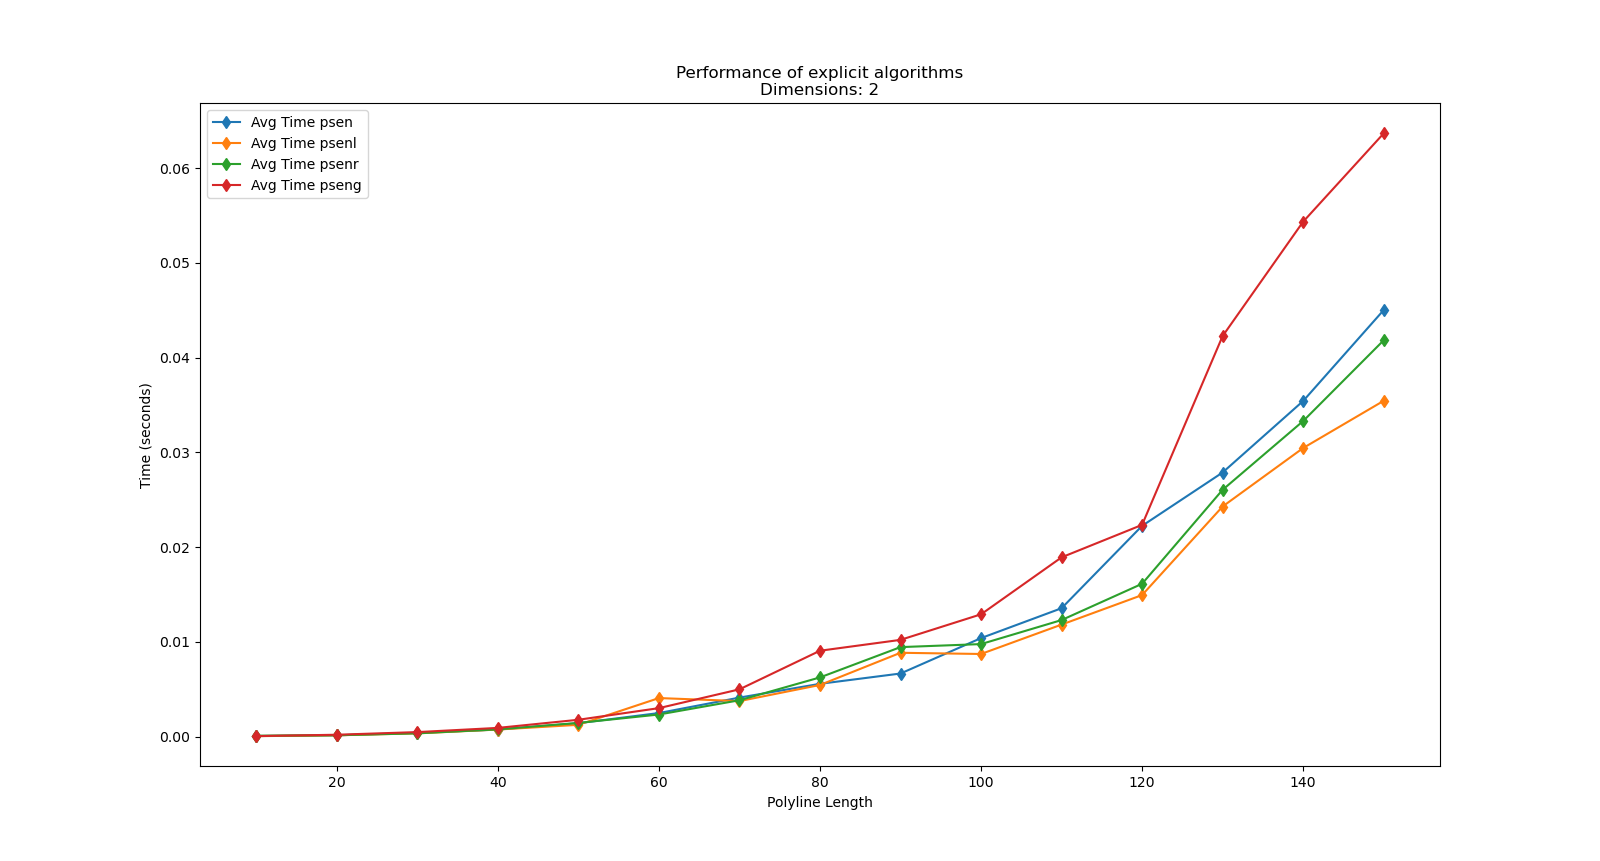
\includegraphics[scale=0.5, width=\linewidth]{figures/psen-opt2.png}
  \caption{Parallel, explicit for well-behaved polylines, comparison of selected optimizations}
  \label{fig:psen-opt2}
\end{figure}

\begin{figure}[ht]
  \centering
  \includegraphics[scale=0.5, width=\linewidth]{figures/psein-opt1.png}
  \caption{Parallel, implicit for well-behaved polylines, comparison of optimizations}
  \label{fig:psein-opt1}
\end{figure}

\begin{figure}[ht]
  \centering
  \includegraphics[scale=0.5, width=\linewidth]{figures/psein-opt2.png}
  \caption{Parallel, implicit for well-behaved polylines, comparison of selected optimizations}
  \label{fig:psein-opt2}
\end{figure}

\section{Conclusions and Future Work}
\label{sec:discussion_conclusion}
We gave a thorough tour through all steps necessary to simplify a polyline using the global Fréchet distance using the algorithm from \citeauthor{on_optimal_polyline_simplification_using_the_hausdorff_and_frechet_distance}. We have extensively discussed how to solve equations involving distance metrics and gave detailed algorithms to solve them for the Manhattan distance, Euclidean distance, and Chebyshev distance. We explained the just mentionend simplification algorithm as well as the algorithm to decide the Fréchet distance decision problem from \citeauthor{computing_the_frechet_distance_between_two_polygonal_curves} for which we provided a simple modified version that is tailored to the given problem. We went through examples for these algorithms to illustrate them and show their geometric intuition and discussed possible optimizations that can be applied. 

Having seen the algorithms, we introduced the implcit and semiexplicit approach to polyline simplification which show that a weaker computational model is sufficient that does not need to take square roots or perform divisons. The semiexplicit approach is an appromative approach that allows easier implementation for general distance metrics. 

Finally, we tested our implementations, showed the results and interpreted them. The explicit approach is more useful in a parallelized setting while the implicit outperforms unparallelized. Surprisingly, the algorithms performed well for relatively long polylines with respect to the theoretical runtime, even without optimizations. 

This leaves many open questions, some of which will be researched in a future thesis. 

\begin{enumerate}
  \item How does the cubic runtime algorithm from \citeauthor{polyline_simplification_has_cubic_complexity_bringmannetal} fare against the optimized versions of the \citeauthor{on_optimal_polyline_simplification_using_the_hausdorff_and_frechet_distance} algorithm? 

    The optimized versions have subquartic runtime but still seem to be slower than cubic runtime. It is possible that the cubic algorithm is worse because of higher constant factors and worse parallelizability. 

  \item Can the space consumption be improved? 

  In the worst case, the polyline simplification algorithm has cubic space complexity. If we only need the size but not the actual simplification itself, it is easy to see that quadratic space suffices. The space can generally be reduced by storing a rooted tree of the triples \((k, i, j)\) which are actually used. An edge in the tree represents one application of the modified Fréchet distance decision problem, meaning we add another shortcut to the simplification. After each layer all nodes on the previously layer which are unused can be trimmed to further reduce space. Such a tree allows inverting the main computation of the algorithm in that we start from the given nodes and find where we can proceed to, instead of iterating over all previous entries to find where we can procede from. The problem is that such a datastructure is less compact as it needs pointers and we still require one layer of quadratic size to efficiently lookup nodes. Further it does not allow for parallelization as easily. 

\item Can simplification be solved in subcubic runtime for the Euclidean distance or small dimensional data? Are there good subcubic approximations?

  \citeauthor{polyline_simplification_has_cubic_complexity_bringmannetal} established a cubic conditional lower bound for the problem which explicitly excludes these cases which are practically the most relevant.

  \item Can simplification be sped up by preprocessing the polyline into a datastructure that allows fast querying?
  
	  This question can already be answered in the affermative, as a simple sorted array with the \(\varepsilon\) intervals that allow simplifications of a certain size can be stored allowing logarithmic querying. However, it is not obvious how to efficiently construct such a datastructure. We think that a sweepline algorithm might work where the events are selected values for \(\varepsilon\). The relevance of this question arises from the cubic conditional lower bound shown by \citeauthor{polyline_simplification_has_cubic_complexity_bringmannetal}. If we cannot improve the runtime for relevant distance metrics or small dimensional data like in the local version of the problem, another way to address the high runtimes preprocessing. 

\item Can the polyline simplification algorithm from \citeauthor{on_optimal_polyline_simplification_using_the_hausdorff_and_frechet_distance} with the outlined optimizations be reanalyzed to have a better theoretical runtime?

  Our experimental data shows that not even quartic runtime is reached so a more sophisticated analysis might yield a better runtime.
\end{enumerate}

